\documentclass[a4paper,oneside,11pt]{report}

\usepackage[T1]{fontenc}
\usepackage{mathptmx}
\usepackage{setspace}
\usepackage{amsmath,amssymb,amsfonts}
\usepackage{graphicx}
\usepackage{subcaption}
\usepackage[numbers]{natbib}
\usepackage{geometry}
\geometry{
	a4paper,
	left=30mm,
	right=30mm,
	top=30mm,
	bottom=30mm 
}
\usepackage{tikz}
\usepackage{blindtext}
\usepackage{etoolbox}
\patchcmd{\abstract}{\null\vfil}{}{}{}
\usepackage[hidelinks]{hyperref}
\usepackage{float}
\usepackage{fixltx2e}
\usepackage{enumitem}
\usepackage{appendix}
\usepackage{pdfpages}

%To make chapter headings higher and to make into one line
\makeatletter
\renewcommand{\@makechapterhead}[1]{%
	{\noindent\raggedright\normalfont% Alignment and font reset
		\huge\bfseries \@chapapp\space\thechapter~~#1\par\nobreak}% Formatting
	\vspace{\baselineskip}% ...just a little space
}
\makeatother

%To start chapter on the same page 
%\makeatletter
%\patchcmd{\chapter}{\if@openright\cleardoublepage\else\clearpage\fi}{}{}{}
%\makeatother

\raggedbottom

\begin{document}
	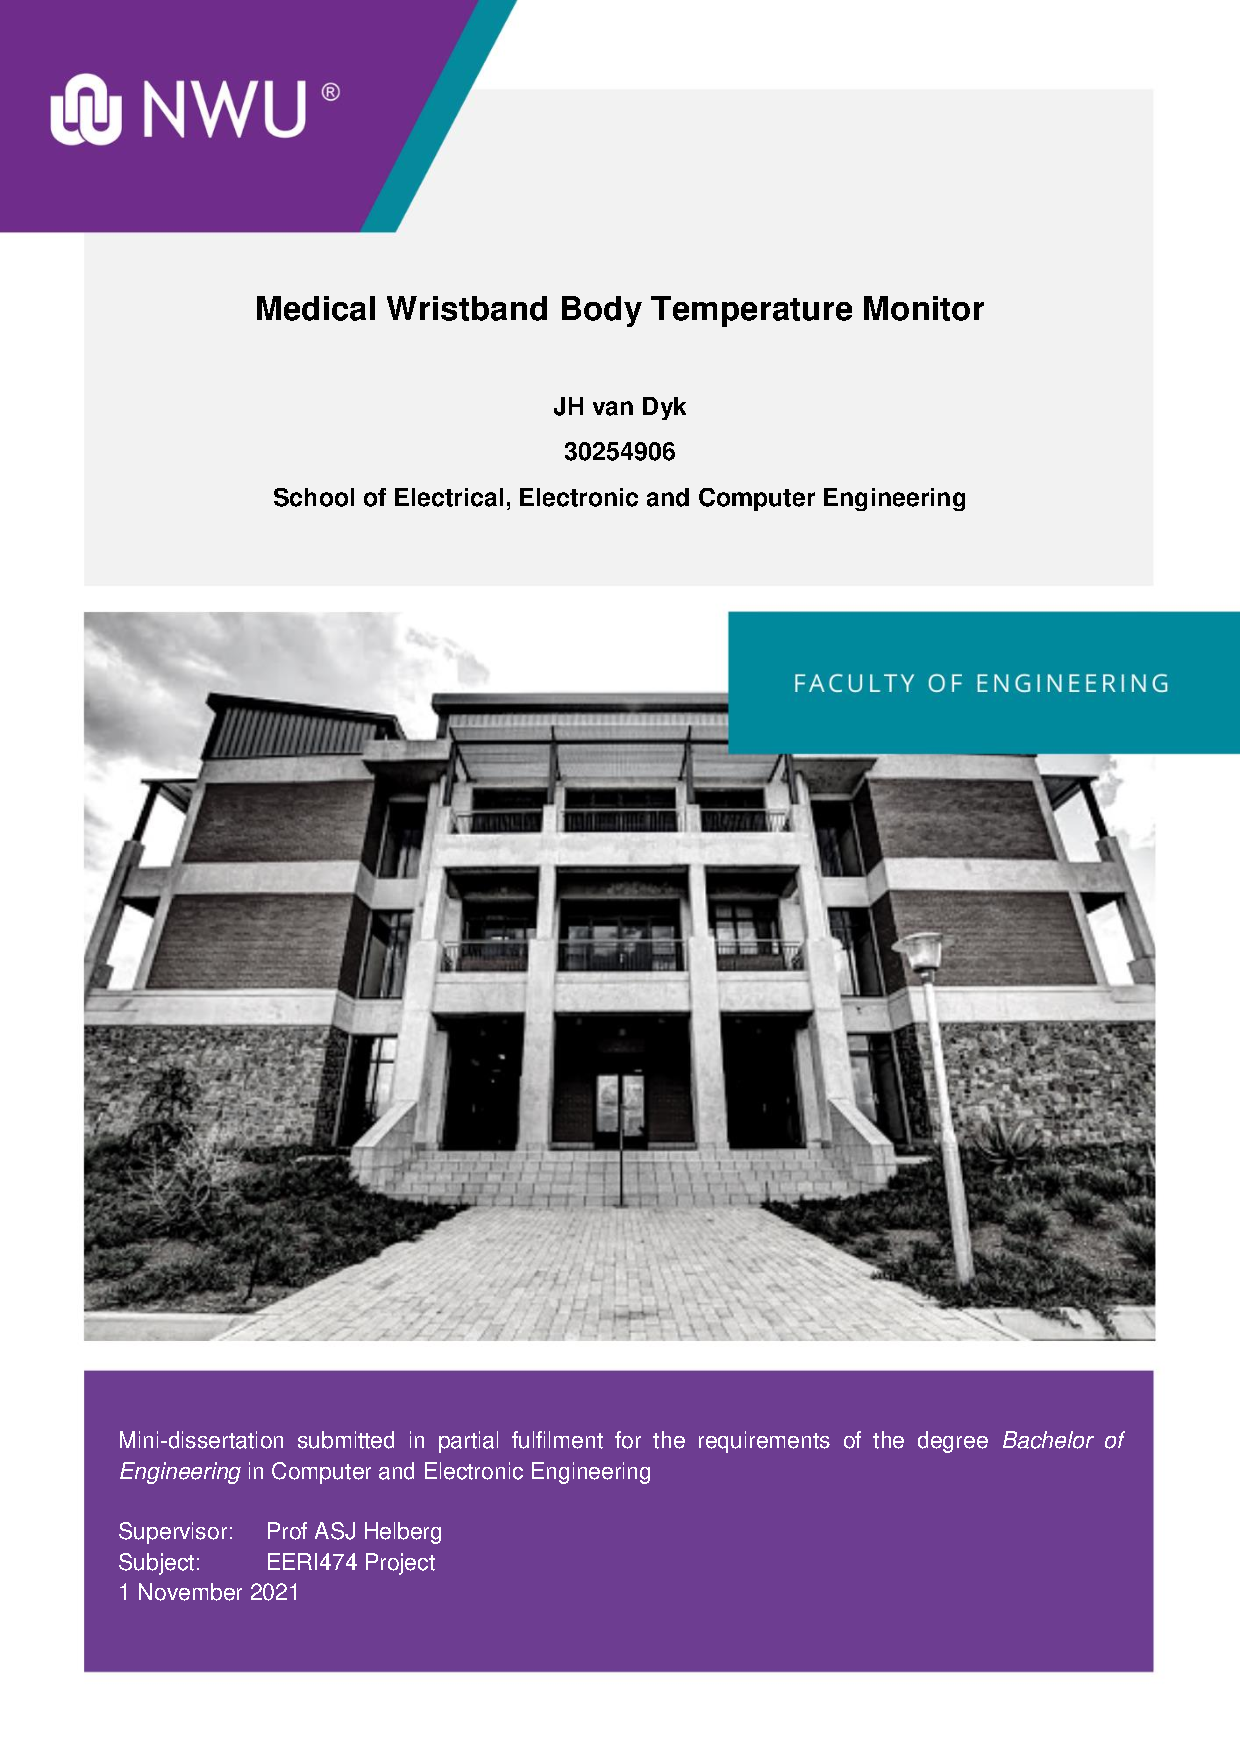
\includepdf[pages=-]{Front-Page.pdf}

	\newpage
	\pagenumbering{roman}
	
	\begin{abstract}
	The following document provides a brief overview on the importance of measuring body temperature. Types of body temperature measuring devices are given to gain an understanding of the context of the problem. The problem is the need for a non-invasive body temperature measuring device that can accurately measure core body temperature, whilst being simple, low-cost, lightweight, and energy-efficient. In the first part of the document, high-level objectives are given that will be pursued in solving the problem. These objectives include the design and implementation of a non-invasive body temperature measuring device, as well as finding a suitable technique to estimate core body temperature from skin temperature. 
	\\
	\\
	A literature study is included in this report to determine what techniques, equipment, technologies, etc. are available to solve the problem. Some background is given on the measurement of body temperature, i.e. where it can be measured and the corresponding difficulties. Since the temperature measured on the skin of a human is susceptible to environmental factors such as surrounding ambient temperatures, four available techniques or methods to accurately estimate core body temperature from the temperature of the skin, are given and reviewed. An overview of the available temperature sensing elements, display technologies as well as power supplies are also given in the literature study.
	\\
	\\
	After the literature study, the design phase is started with the conceptual design of the Body Temperature Monitoring device. A Model-based Systems Engineering (MBSE) process is followed throughout the design phase. A functional analysis is used to clearly state how the system is to work when fully completed, followed by an architectural synthesis where the physical design of the device is developed. Once the conceptual design was completed, the detailed design of the device started. Trade-off studies were used to select the specific components to construct the device. Multi-Criteria Decision Matrices (MCDM) are used in the decision-making process to ensure no subjectivity or bias would affect the outcome of the selection of the components. Once all the required components were selected, the full detailed design of the device is presented in the form of schematics. The firmware is developed in the embedded C programming language, and a Finite State Machine (FSM) representation, as well as software flow diagrams, are provided to visualise the design and logical flow of the firmware that will be flashed onto the device.
	\\
	\\
	The detailed design was then implemented and tested. A prototype PCB was designed and constructed to test if the device functions as intended. Firstly the communication between the programmer and the microcontroller was tested, and the programmer could successfully communicate with the microcontroller of the device. This means that program code could be flashed onto the device. After this, the accuracy with which the device measures skin temperature was determined and was found as $ 98.32 \% $ at its lowest, relating to a $ 0.5^{\circ} C $ maximum error when measuring skin temperature. The accuracy with which the device estimates the core body temperature from the skin temperature was also determined, and was found as $ 98.39 \% $ at its lowest, relating to a $ 0.58^{\circ} C $ maximum error when estimating body temperature. The power consumption of the device was then measured to estimate the battery life of the device. If the device is used twice every hour, for 10 seconds, the estimated battery life of the Body Temperature Measuring device is 212.34 days. The final findings are then documented in the conclusion to test if all the requirements were met during the project. It is concluded that the designed Body Temperature Measuring device is an accurate, small, lightweight device whilst being energy efficient and cheap to construct. The concluding chapter also gives a few recommendations regarding further development.
		
	\end{abstract}
	\tableofcontents
	\newpage
	\listoffigures
	\newpage
	\listoftables
	\chapter*{List of Abbreviations}

\begin{table}[H]
	\begin{tabular}{ll}
		\textbf{\Large HMI} & \large Human-Machine Interface\\
		\textbf{\Large MBSE} & \large Model-Based Systems Engineering\\
		\textbf{\Large MCDM} & \large Multi-Criteria Decision Matrix\\
		\textbf{\Large WPM} & \large Weighted Product Method\\
		\textbf{\Large CAD} & \large Computer-Aided Desig\\
		\textbf{\Large CBT} & \large Core Body Temperature\\
		\textbf{\Large I2C} & \large Inter-Integrated Circuit\\
		\textbf{\Large SCL} & \large Serial Clock Line\\
		\textbf{\Large SDA} & \large Serial Data Line\\
		\textbf{\Large ADC} & \large Analog-to-Digital Converter\\
		\textbf{\Large GPIO} & \large General-Purpose Input/Output\\
		\textbf{\Large RAM} & \large Random Access Memory\\
		\textbf{\Large RTC} & \large Real-Time Clock\\
		\textbf{\Large SWD} & \large Serial Wire Debug\\
		\textbf{\Large ISR} & \large Interrupt Service Routine\\
		\textbf{\Large FSM} & \large Finite State Machine\\
		\textbf{\Large DC} & \large Direct Current\\
		\textbf{\Large IC} & \large Integrated Current\\
		\textbf{\Large PCB} & \large Printed Circuit Board\\
		\textbf{\Large LED} & \large Light-Emitting Diode\\
		\textbf{\Large OLED} & \large Organic Light-Emitting Display\\
		\textbf{\Large LPD} & \large Laser Phosphor Display\\
		\textbf{\Large ELD} & \large Electroluminescent Display\\
		\textbf{\Large TFT} & \large Thin-Film-Transistor\\
		\textbf{\Large NTC} & \large Negative Temperature Coefficient\\
		\textbf{\Large PTC} & \large Positive Temperature Coefficient\\
		\textbf{\Large RTD} & \large Resistive Temperature Detector\\
	\end{tabular}
\end{table}

	\newpage
	
	\setcounter{page}{1}
\pagenumbering{arabic}
\chapter{Introduction}\label{Ch1}

\section{Purpose of document}
This report covers the context in which a problem exists and also why it is important to address the problem by providing a short background on devices that measure body temperature, the use thereof, and the working of these devices. Some background information is then used to provide a summary of the problem at hand. A possible solution is then shortly discussed, followed by some high-level objectives that will be pursued in an attempt to solve this problem. Anticipated benefits of the solution, technical requirements, scope of the project, and project deliverables are given to provide more context of this project. 


\section{Background}
Body temperature can be defined as the measure of how well the human body can get rid of and generate heat. Body temperature is needed to sustain and promote human life. The measurement of body temperature plays an important role in our everyday life (especially in the pandemic we find our-self in) since several diseases are characterised by a change in body temperature. Some body temperature measuring devices, such as the clinical thermometer, which is commonly used domestically and in hospitals, must be placed underneath one's tongue or under the armpit. This proves to be unhygienic when these measuring devices are not properly cleaned and can also cause some annoyance for certain people. The need for non-invasive body temperature measuring equipment exists, that can fast and effectively determine body temperature on the move. Mobility will ensure that body temperature readings are always available, anywhere. 
\\
\\
Rotational motions and constant internal vibrations in molecules generate thermal energy or heat. Temperature is therefore a measure of the average thermal energy of molecular motions. Biochemical processes take place inside living cells that contain molecules and are greatly influenced by body temperature \cite{Chen2019}. These biochemical processes are known as metabolism. Humans are homeothermic and body temperature is regulated at about 37°C ± 1°C \cite{Wong2015}. The body needs to maintain its temperature at a certain level to support and stimulate its metabolic activities. Both temperature statuses, hyperthermia (too high) or hypothermia (too low) can alter metabolic activities, cause tissue damage and disturb organic functions. Hence, it is important to examine and monitor body temperature to hunt for signs of diseases that are characterised by a change in body temperature. Body temperature measurements allow doctors and other medical practitioners to analyse the effectiveness of the prescribed treatment. 
\autoref{tab:1} shows both extremes of body temperature and some associated effects at certain temperatures. 

\begin{table}[H]
	\centering
	\caption{\textit{Body temperature effects}\cite{Chen2019}}
	\label{tab:1}
	\begin{tabular}{|c|c|}
		\hline
		\textbf{Temperature} & \textbf{Effect}\\
		\hline
		\hline
		24-28°C & Mostly death.\\
		\hline
		29-33°C & Sleepiness, slow heartbeat, moderate to severe confusion, unresponsive to stimulus.\\
		\hline
		34-35°C & Bluish/Grayness of the skin, intense shivering, numbness and some confusion.\\
		\hline
		36°C & Mild to moderate shivering.\\
		\hline
		37°C & Normal temperature.\\
		\hline
		38-40°C & Dehydration, headache, vomiting and severe sweating.\\
		\hline
		41-42°C & Confusion, fainting, very fast heart rate and high/low blood pressure.\\
		\hline
		43°C & Brain damage, normally death.\\
		\hline
	\end{tabular}
\end{table}
\noindent
Various types of body temperature measuring devices already exist. Some of the most popular domestic-used devices are listed below, each followed by a short description:
\begin{itemize}
	\item Oral Thermometer:\\Most oral thermometers are digital with a housing made out of plastic. This is an invasive device that must be placed under the tongue for a short while allowing it to measure body temperature. The oral thermometer uses thermistor resistance that varies with temperature as sensing element. In many cases, the user will be alerted when the reading is completed. 
	\item Tympanic Thermometer:\\Tympanic Thermometers are minimally invasive since it is placed inside the ear canal to take body temperature readings. This type of device measures the natural emission of infrared thermal radiation from the	tympanic membrane. This digital device has a cone shape designed to fit into an ear. 
	\item Mercury-in-glass/ Alcohol-in-glass Thermometer:\\ This device measures oral, rectal, or armpit body temperature through the thermal expansion of ethanol/mercury. These types of devices are made of glass and the thermal expansion of the ethanol/mercury caused by heat must be noted by the user when taking a reading. 
	\item Infrared Thermometer:\\This is a non-invasive device that measures thermal radiation (infrared) emitted from the forehead and skin to deduce body temperature. The infrared thermometer uses a pyroelectric sensor to measure temperature. Infrared thermometers provides a digital temperature reading and the user could be alerted when this reading is abnormal. 
\end{itemize}
The devices listed have their own advantages and disadvantages. According to \cite{Whelan2020}, oral thermometers are most accurate for children over 3 years of age and adults. The drawback is that, as mentioned earlier, if the device is not cleaned properly it may be unhygienic. The article also mentions that tympanic thermometers provide fast and accurate readings but objects such as earwax and improper positioning may distort results. The Mercury-/Alcohol-in glass thermometers are not digital devices, the user must constantly look at the expansion of the liquid to determine the reading. Infrared thermometers provide quick readings contactless. However, it is believed that these infrared thermometers are not truly as accurate as the rest since external factors, such as direct sunlight and indoor heating, may affect the readings \cite{Whelan2020}.
\\
\\
Throughout this section, mentions of invasive and non-invasive methods were made. These are the two main methods to measure body temperature — by measuring core (deep tissue, invasive) temperature and surface (skin, non-invasive) temperature. Invasive temperature measurements can be taken through the oral cavity, ear canal, and rectum, whilst non-invasive readings are made on the skin surface. In many cases invasive methods cannot be used, such as when someone is unconscious, confused, or sneezing repeatedly, then the oral measurement method is unsuitable. When someone has a middle ear infection or an obstruction in their ear by wax, the ear method is of no use. Non-invasive methods can easily be affected by external factors such as sunlight and indoor heating/cooling. 
\section{Problem Statement}
From the previous section, it is clear that a non-invasive body temperature measuring device is needed that can measure core body temperature, without the readings getting affected by external factors, whilst being comfortable. 

\section{Hypothesis}
A medical wristband that can measure body temperature will be designed and constructed. This allows end-users to wear the device on their wrist, and to see his or her body temperature that is measured and displayed by the wristband. 

\section{Project Objective}
\subsection{Primary Objective}
The primary objective of this project is to design an accurate body temperature measuring device that can be worn as a wristband. The device should measure one's body temperature without the readings getting affected by external factors. The device will predict core body temperature instead of just measuring surface (skin) temperature. 
\\
\\
Since the device will predict core body temperature, a thermal equivalent circuit model will be used to measure core body temperature with a skin-attachable sensor and experimental investigations will be used to further improve this model. Improvements will lead to more accurate readings. A low-level example of a thermal equivalent circuit model can be seen in \autoref{fig:1}.
\begin{figure}[!htbp!]
	\centering
	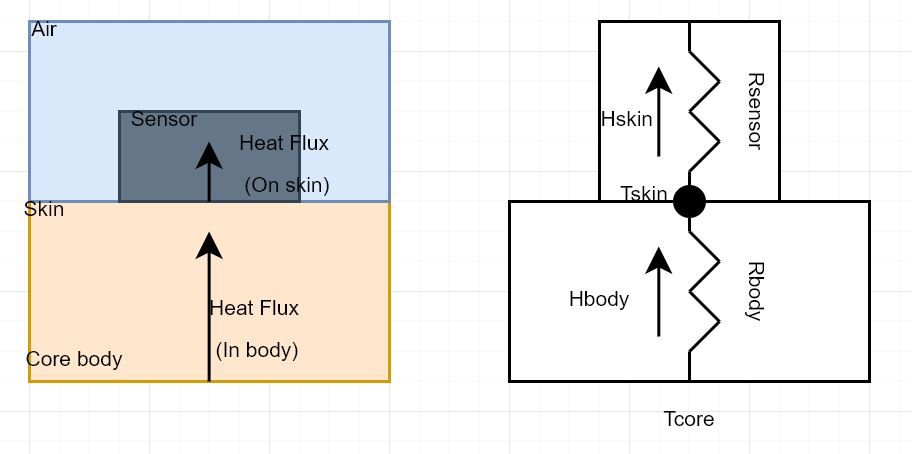
\includegraphics[scale=0.5]{img/Temp_Model}
	\caption{Low level model and thermal equivalent circuit.}
	\label{fig:1}
\end{figure}

\subsection{Secondary Objective}
The device will be able to measure body temperature, this must also be displayed to the user of the wristband. Therefore, the secondary objective is to implement a Human-Machine Interface (HMI). 

\section{Anticipated Benefits of Solution}
The device in the form of a wristband will make the process of measuring body temperature easier and more efficient since the wristband can be comfortably worn throughout the day or night providing continuous readings. These readings are updated by the device on a set interval or on-demand, whilst always displaying the most recent reading. Users will be alerted when the temperature is too high or low so that the necessary steps can be taken right away. This will also be a low-cost, yet reliable build.  

\section{Technical Requirements}\label{1.7}
\subsection{Requirements}
The requirements are listed below:
\begin{enumerate}
	\item Lightweight. The final wristband with the measuring device and the HMI shall be lightweight. This supports the need for a comfortable device. 
	\item Low energy usage. Since the end product will be in the form of a wristband, it will be portable. This means that the measuring device will be battery-powered. Low energy usage shall extend the battery life of the device. 
	\item Cheap. The low-cost aspect of the end product will ensure that the wristband can be widely used by anyone with the need. 
	\item Simple. The device will measure body temperature, show the measured temperature and alert the user when the temperature is outside the set limits.
	\item Accurate. The device shall deliver readings with an accuracy of $\pm$0.5°C to the user of the device. 
	\item The measuring range of the device shall be from 30°C to 40°C, since these temperatures are roughly the limits any living person will achieve.  
	\item The device shall operate in atmospheric temperatures ranging from -5°C to 45°C, making the body temperature measuring device operational in the summer and winter.  
\end{enumerate}

\subsection{Scope Definition}
The scope of the project is to design and implement a body temperature measuring device that can report back a measured reading. Therefore, the sensing element, power supply or battery, and HMI components will not be re-designed, existing components will be used and placed on a Printed Circuit Board (PCB) to make the device small and compact. The wristband itself will not be part of the design, although this can be 3D printed. 

\section{Deliverables}
A device that can measure and display body temperature on the move by placing the device on the wrist will be delivered. This device will be mounted on a wristband that can fit around one's arm at the wrist. Circuit design and PCB layout, together with an enhanced thermal equivalent circuit, or another technique to estimate core body temperature from skin temperature, will also be provided. 

\section{Concluding Remarks}
This section explained the importance of measuring body temperature as it is an indication of a person's physical health status. Some requirements are given, showing what will be incorporated in the final product. The scope definition ensures that all the requirements are reached without doing unnecessary work. 
	\chapter{Literature Study}\label{Ch2}
This chapter contains a literature study on the most relevant techniques, equipment, and technologies related to this project. Firstly a high-level block diagram of the proposed solution is given where-after the relevant technologies that are commonly available within the scope of the proposed solution are discussed. The different types of temperature transducers, display, and battery technologies related to this project are reviewed and some important methods to measure core body temperature from skin temperatures are discussed. 

\section{High-level block diagram}
In this section a high-level block diagram of the proposed solution is given. The diagram is shown in \autoref{fig:8} and consists of 4 main functional units. 
\begin{figure}[H]
	\centering
	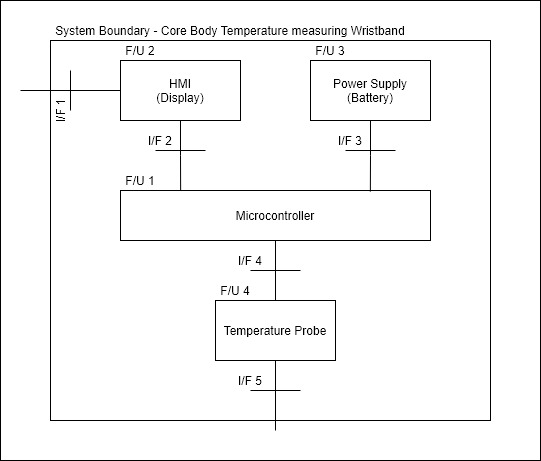
\includegraphics[scale=0.7]{img/High-level-block-diagram}
	\caption{High level block diagram of proposed solution}
	\label{fig:8}
\end{figure}
\noindent
The functional units of the proposed solution are briefly discussed in \autoref{tab:3}.
\begin{table}[H]
	\centering
	\caption{\textit{High-level functional unit description}}
	\label{tab:3}
	\begin{tabular}{|p{8cm}|p{4cm}|}
		\hline
		\textbf{Description} & \textbf{Functional Unit}\\
		\hline
		Analogue to Digital conversion, Processing and analysis of measurements, estimation of core body temperature. & Microcontroller\\
		\hline
		Display the measured temperature. & HMI\\
		\hline
		Deliver power to the system. & Power Supply\\
		\hline
		Measure skin temperature, configuration will allow the microcontroller to estimate core body temperature. & Temperature Probe\\
		\hline
	\end{tabular}
\end{table}

\section{Classification of Body Temperature}
Body temperature measuring dates back to ancient times when physicians used their hands to estimate body temperature by noting the difference in temperature between the head and foot of a patient. As society modernised, more information and technology became available, leading to instruments that can predict and measure body temperature. In practice, the measurement of body temperature is categorised in three distinct types referred to as core body temperature, surface body temperature, and basal body temperature \cite{Chen2019}. The type is determined by considering measurement position. Core body temperature refers to the deep tissue of the body and is the operating temperature of all inner organs. Core body temperature is measured using invasive methods. Surface body temperature is measured on the skin and can be used to estimate core body temperature. Basal body temperature is the lowest body temperature taken right after waking up and before any physical activity and is mostly used to determine and predict ovulation in women \cite{Basal}. There are different places available to measure the body temperature of a human such as sublingual, esophagus, bladder, rectum, and digestive tract for the measurement of core body temperature, and axilla, groin, neck, and wrist for surface body temperature. \\\\
Surface body temperature can easily be measured non-invasively, but can also be susceptible to environmental factors. Since there is a need for a non-invasive body temperature device, the rest of the literature study will focus on surface body temperature measuring techniques, sensing elements, and how to predict core body temperature from surface body temperature. 

\section{Temperature sensing elements}
Temperature sensing elements, or from now on referred to as transducers, convert heat energy or temperature into other forms of energy \cite{Chen2019}. The other forms of energy can then be processed and the temperature can be made visible on a legible temperature scale. This section discusses several temperature transducers that can be used to measure core body temperature. 

\subsection{Thermistor}
Thermistors are semiconductor-resistive temperature transducers where the resistance of the material changes as the temperature changes \cite{Gums2018}. There are two types of thermistors available, the Negative Temperature Coefficient (NTC) thermistor and the Positive Temperature Coefficient (PTC) thermistor \cite{Borwankar2015}. The resistance of an NTC thermistor decreases as the temperature increases and consequently the resistance of a PTC transducer increases as the temperature increases. NTC thermistors are commonly used in body temperature measurements since it has good linearity in the range of body temperature, whereas the PTC thermistor has poor sensitivity in the range of body temperature and are mostly used for higher temperature measurements \cite{Chen2019}. The conversion from resistance to temperature is usually given in the datasheet of the specific thermistor. 

\subsection{Thermocouple}
Thermocouples have two different metal wires connected together as a junction and when the temperature of the junction is changed, the junction output voltage varies with this change \cite{Nookhao2020}. Therefore, the Seebeck effect is used as a thermoelectric transducer \cite{Chen2019}. The Seebeck effect is the phenomenon in which a temperature difference of two dissimilar conductors connected together produces a voltage gradient. This voltage can then be measured and converted to temperature. Several types of thermocouples are available and are classified according to the conductor alloy used inside the thermocouple \cite{Gums2018}. The different types are differentiated by designated letters. Some of the most commonly used thermocouples are shown in \autoref{tab:2}.
\begin{table}[H]
	\centering
	\caption{\textit{Thermocouple types \cite{Maxim2017}}}
	\label{tab:2}
	\begin{tabular}{|c|c|c|}
		\hline
		\textbf{Designated letter} & \textbf{Conductor Alloys (+/-)} & \textbf{Sensing Range (°C)}\\
		\hline
		E & Nickel Chromium / Constantan & -40 to 900\\
		\hline
		J & Iron / Constantan & -180 to 800\\
		\hline
		K & Nickel Chromium / Nickel Aluminium & -180 to 1300\\
		\hline
		N & Nicrosil / Nisil & -270 to 1300\\
		\hline
		T & Copper / Constantan & -250 to 400\\
		\hline
		R/S & Copper / Copper Nickel Compensating & -50 to 1750\\
		\hline
		B & Platinum Rhodium & 0 to 1820\\
		\hline
	\end{tabular}
\end{table}
\noindent
Most applications that use a thermocouple as a temperature transducer, require precise amplification since the output voltage is quite small. This adds circuitry to the measurement device and is not ideal for smaller-sized projects.

\subsection{Resistive Temperature Detector}
Resistive Temperature Detectors or RTDs work on the same principle as thermistors, where the varied resistance of the metal is measured when there is a temperature change. The most common and accurate material used to make RTDs is platinum \cite{Gums2018}. The reason for this is that platinum RTDs offer a nearly linear response to temperature changes, repeatable responses, a wide temperature range, and they are accurate and stable. RTD configurations can be two-/three-/four-wire and is shown in \autoref{fig:2}. An excitation current flows through the RTD and the voltage across the RTD is measured.
\begin{figure}[H]
	\centering
	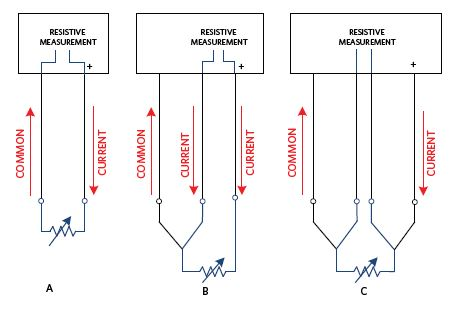
\includegraphics[scale=0.7]{img/RTD-configurations}
	\caption{RTD configurations \cite{Maxim2017}}
	\label{fig:2}
\end{figure} 
\noindent
RTD thermal transducers respond slower than thermocouples to changes in temperature \cite{Gums2018}.

\subsection{Semiconductor based Integrated Circuit}
The semiconductor sensor in an integrated circuit (IC) contains many types of circuitry on one chip \cite{Nookhao2020}. Semiconductor-based IC measures temperature by using the physical properties of a transistor \cite{Gums2018}. The collector current and base-emitter voltage of a bipolar junction transistor (BJT) is used to calculate the measured temperature. The PN junction is therefore used as a temperature transducer. The forward voltage drop across a forward-conducting PN junction of a transistor at constant forward-bias current exhibits linear temperature dependence over a wide temperature range \cite{Chen2019}. Temperature transducers based on this principle can be realised by applying a square-wave current to a PN junction \cite{Verster1968} or by using two matched devices operating at different currents. 

\subsection{Infrared}
The temperature of an object can be measured by the thermal radiation power emitted from the object if the object has a temperature above absolute zero (0 Kelvin). The infrared energy emitted from an object is proportional to its temperature. This method can be used to measure body temperature since the peak of the thermal radiation emitted from a human body lies in the far-infrared region \cite{Chen2019}. The infrared type temperature transducer can make temperature measurements contactless. Most infrared temperature transducers use a pyroelectric sensor to measure temperature. 


\section{Techniques for Non-invasive CBT measurements}\label{Sec2_4}
Several non-invasive methods have been developed to measure core body temperature since the early 1970s \cite{Chen2019}. The reason for this is that some core body temperature measuring techniques are unsatisfactory for continuous use and may cause discomfort to the patient \cite{Yamakage2003}. Furthermore, some invasive measurements can induce complications \cite{complications}. The working of the developed methods is discussed next. 

\subsection{Zero-heat-flow Method}
The zero-heat-flow method is used to estimate core body temperature in a non-invasive manner. The estimation is made by measuring the temperature on the skin surface with a probe that consists of two thermistors, a thin-film heater element, and a piece of nylon used as a thermal insulator. These components are encapsulated by silicone rubber and the structure can be seen in \autoref{fig:3}.
\begin{figure}[H]
	\centering
	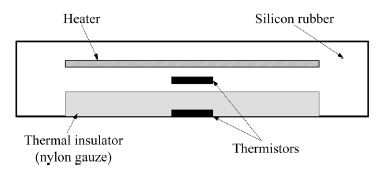
\includegraphics[scale=0.8]{img/zero-heat-flow}
	\caption{Zero-heat-flow structure\cite{Chen2019}}
	\label{fig:3}
\end{figure} 
\noindent
The heater element is used to reduce ambient effects on measurements \cite{Matsunaga2020}. The method is based on heat or thermal insulation to reduce heat loss from the skin. Two matched thermistors are used to detect the temperature on both sides of the insulating layer and these temperatures are then compared. The temperature difference between them is used to control the heater current in such a way that there is no temperature gradient across the insulating layer, therefore no heat flowing through this layer \cite{Yamakage2003}. As long as the condition of zero-heat-flow is satisfied, the probe can be seen as an ideal thermal insulator, and heat loss from the skin is prevented. After a while (around 15 minutes), the skin temperature will be in equilibrium with deep tissue temperature and the lower thermistor that is in contact with the skin may be used to measure skin temperature \cite{Yamakage2003}.
\\
\\
Since a heater element is present in this method, it requires a substantial amount of power. This, together with the relatively big size is not ideal for low-energy, smaller-sized projects.

\subsection{Dual-heat-flux Method}
In response to the zero-heat-flow method mentioned above that needs a heater element, the dual-heat-flux method was developed that works without a heating element \cite{Kitamura2010}. The measurement probe is built structurally to form two different thermal pathways, hence the name dual-heat-flux. Temperature is measured by temperature transducers at the end of each channel. The structural layout of this method is shown in \autoref{fig:4}.
\begin{figure}[H]
	\centering
	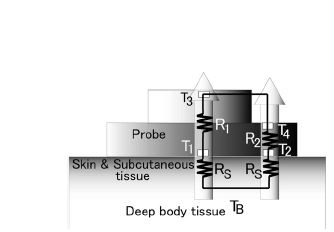
\includegraphics[scale=0.9]{img/dual-heat-flux}
	\caption{Dual-heat-flux structure\cite{Kitamura2010}}
	\label{fig:4}
\end{figure} 
\noindent
From the schematic diagram above, the two channels of heat flow and the equivalent circuit can be seen. The skin is covered by two kinds of heat insulators that have different thermal resistances, $R_{1}$ and $R_{2}$, $R_{s}$ is the thermal resistance of the subcutaneous tissues and skin, $T_{1}$ and $T_{2}$ are the skin temperatures under the insulator, and $T_{3}$ and $T_{4}$ are the upper temperatures at the surface of the insulator \cite{Chen2019}. $T_{B}$ is the core body temperature that needs to be measured. Kitamura et al. \cite{Kitamura2010} derived the following equation to estimate core body temperature by assuming that $R_{s}$ of both channels are identical:
\begin{equation}
	T_{B} = T_{1} + \frac{(T_{1} - T_{2})(T_{1} - T_{3})}{K(T_{2} - T_{4})(T_{2} - T_{4})}
	\label{1}
\end{equation}
\noindent
$K$ is the ratio of thermal resistance and can be determined from \autoref{1} by rearranging the terms and conducting experimental calibration in a water bath:
\begin{equation}
	K = \frac{(T_{B} - T_{2})(T_{1} - T_{3})}{(T_{B} - T_{1})(T_{2} - T_{4})}
\end{equation}
where, $T_{B}$ can be set to the preset water temperature. 
\\
\\
This method has shown promising results, however, underlying skin anatomy and ergonomics still remain an issue \cite{Atallah2018}. In this method $R_{s}$ of both channels are presumed to be identical since two insulators are placed close to each other, resulting in $K$ not being influenced by $R_{s}$. However, Feng et al. \cite{Feng2017} found that $K$ is a function of the thickness of the skin or body, and $R_{s}$ cannot be cancelled out once $R_{s}$ changes. $R_{s}$ will change with different skin types, colours, and thicknesses. Feng et al. \cite{Feng2017} also revealed that the dual-heat-flux method has a long measurement time and systems based on this method are relatively large.

\subsection{Thermal equivalent circuit model}
The dual-heat-flux method does not take ambient conditions into consideration and heat flux from core body temperature may uncontrollably leak directly into the ambient environment instead of being measured by the transducers mentioned in the dual-heat-flux method \cite{Matsunaga2020}. Another method to measure core body temperature from the skin surface is to use the thermal equivalent circuit model to estimate core body temperature with a skin-attachable probe. 
\\
\\
The thermal equivalent circuit for a skin-attachable sensor for the core body temperature estimation model was first developed by Fox et al. \cite{Fox1973}. An amended thermal equivalent circuit can be seen in \autoref{fig:1} of this report. The core body temperature ($T_{core}$) is estimated by the following:
\begin{equation}
	T_{core} = T_{skin} + (R_{body} \times H_{skin})
\end{equation}
where the skin surface temperature, the measured heat flux and the thermal resistance of the body are denoted by $T_{skin}$, $H_{skin}$ and $R_{body}$ respectively. Matsunaga et al. \cite{Matsunaga2020} developed an improved thermal equivalent circuit model which takes the uncontrolled heat flux leak to the ambient environment, and external convection changes into consideration. The improved thermal equivalent circuit is shown in \autoref{fig:5}.
\begin{figure}[H]
	\centering
	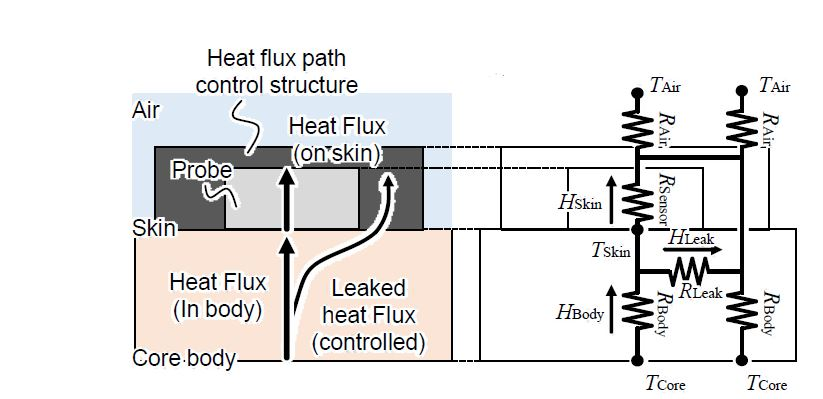
\includegraphics[scale=0.6]{img/improved-temp-model}
	\caption{Improved thermal equivalent model \cite{Matsunaga2020}}
	\label{fig:5}
\end{figure}
\noindent
In this figure, the thermal resistance of the probe, heat flux in the body, the ambient temperature, and thermal resistance to ambient air are denoted by $R_{sensor}$, $H_{body}$, $T_{air}$ and $R_{air}$ respectively. $R_{leak}$ and $H_{leak}$ denote the thermal resistance of the leakage path and the leaked heat flux. Matsunaga et al. \cite{Matsunaga2020} then gives the core body temperature ($T_{core}$) as the following:
\begin{equation}
	T_{core} = T_{skin} + (R_{body} \times \alpha H_{skin})
\end{equation}
\noindent
$\alpha$ is the calibration coefficient and is given by:
\begin{equation}
	\alpha = \frac{(H_{skin} + H_{leak})}{H_{skin}}
\end{equation}
\noindent
By using $H_{skin}$ and $H_{leak}$ together with Kirchhoff's first and second laws, $\alpha$ can be rewritten as a function of thermal resistance:
\begin{equation}
	\alpha = 1 + \frac{R_{sensor}}{R_{leak}}
	\label{6}
\end{equation}
\noindent
From \autoref{6} it is clear that $\alpha$ does not depend on $R_{air}$ which means that the calibration coefficient does not change by changes in ambient conditions, and consequently, estimation errors do not occur. Through this process, Matsunaga et al. \cite{Matsunaga2020} considered $R_{body}$ and $R_{leak}$ as constant since they mainly depend on the thickness of the human body at the point of measuring. $R_{sensor}$ is also constant. To control the heat flux path, the probe is wrapped with a highly conductive material to ensure that the leaked heat flux is passing through the thermally conductive material. 
\\
\\
It is clear that the thermal resistance of the body is still needed to use this method. When using an average value for $R_{body}$ estimation errors may occur that impacts the accuracy of the method. It is also generally quite difficult to obtain the thermal resistance of the leakage path. 

\subsection{Statistical Estimation}\label{stat}
This method estimates core body temperature from skin temperatures by following a  technique that is completely different from the previous methods. Kwak et al. \cite{Kwak2019} proposed a statistical estimation of core body temperature from skin temperature. In this method, the central limit theorem of statistics is used to overcome the problems faced when using a skin-attachable sensor to measure core body temperature. One of the major problems that are faced is that skin temperature is affected by external conditions such as wind and ambient temperature. The central limit theorem states that if there is a population with a mean and a standard distribution and many samples are taken from the population, the distribution of the sample means will be approximately normally distributed \cite{Sang2017}. In other words, arbitrary distributions are normally distributed as the number of samples increases. Kwak et al. \cite{Kwak2019} uses this theorem to obtain a normal distribution of skin temperature and core body temperature and map each normal distribution to each other. 
\\
\\
This method requires a lot of data or samples to increase its accuracy. Therefore, many measurements should be made on the ambient temperature, the skin temperature and the core body temperature. After a generous amount of data is gathered, the statistical model can be build. The following steps are followed to build the statistical model \cite{Kwak2019}:
\begin{enumerate}
	\item Draw boxplot:\\
	A boxplot is a standard way of showing the distribution of data by providing a five number summary(minimum, first quartile, median, third quartile, and maximum). Outliers from the data model based on core body temperature are excluded since some measurements may be erroneous. 
	\item Draw histograms:\\
	A histogram of skin temperature and core body temperature should be drawn respectively. The histograms are then used to find the fitting Gaussian functions for skin temperature and core body temperature. The Gaussian functions for skin temperature and core body temperature are respectively:
	\begin{eqnarray}
		skin\_gauss(x) = a_{1} \times \exp [-(\frac{x-a_{2}}{a_{3}})^2]\\
		body\_gauss(y) = b_{1} \times \exp [-(\frac{y-b_{2}}{b_{3}})^2]
	\end{eqnarray}
	where $x$ is a random variable for skin temperature, $y$ a random variable for core body temperature, $a_{1}$, $b_{1}$ the amplitudes, $a_{2}$, $b_{2}$ the centroids and $a_{3}$, $b_{3}$ the peak widths. 
	\item Map the Gaussian function of skin temperature to the Gaussian function of core body temperature:\\
	The Gaussian function of skin temperature is firstly mapped to a standard normal distribution and then the standard normal distribution is mapped to the Gaussian function of core body temperature. A relevant example of the mapping is shown in \autoref{fig:6}.
	\begin{figure}[H]
		\centering
		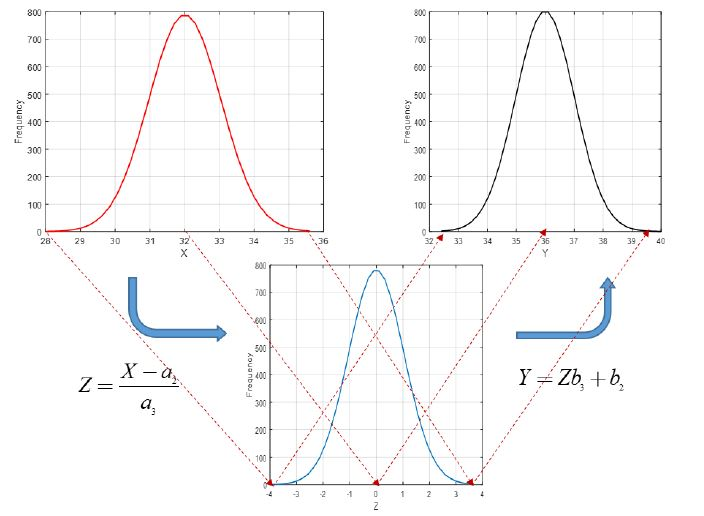
\includegraphics[scale=0.5]{img/stats-mapping}
		\caption{Mapping of Gaussian functions \cite{Kwak2019}}
		\label{fig:6}
	\end{figure}
	\noindent
	where the corresponding formula is given by:
	\begin{equation}
		Y = b_{3}(\frac{X - a_{2}}{a_{3}}) + b_{2}
	\end{equation}
\end{enumerate}
\noindent
Kwak et al. \cite{Kwak2019} concluded that the statistical method estimates core body temperature reliably and that the estimated core body temperatures are within the margin of error tolerance of actual thermometers. The main drawback of this method is that a lot of data or samples are needed to build a statistical model that will deliver reliable results. 


\section{Display Technologies} 
Many display technologies and modules coexist and compete for their share in the market \cite{Fer2015}. The term display in this context is referring to an output device that can exhibit, show or project information to visually communicate with a user. This section will focus on the most widely used display technologies that are available for low power consumption applications.
\\
\\ 
Fernández et al. \cite{Fer2015} reviewed the display technologies available, focusing on the power consumption of each technology. The following figure shows the power consumption density of the various display technologies:
\begin{figure}[H]
	\centering
	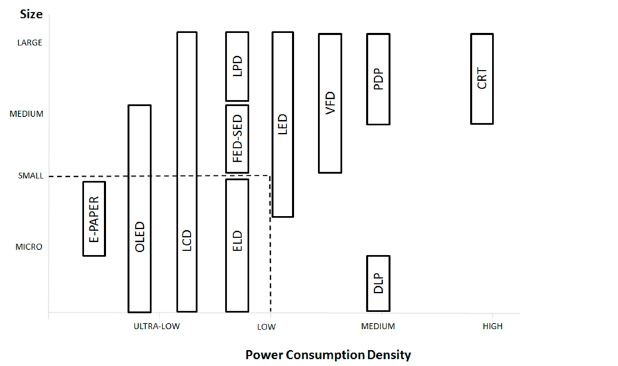
\includegraphics[scale=0.9]{img/Display-power}
	\caption{Power Consumption Density of Display Technologies \cite{Fer2015}}
	\label{fig:7}
\end{figure}
\noindent
From \autoref{fig:7} the technologies that consume low, and ultra-low power can be determined. These display technologies that are commonly used will be briefly discussed next. 

\subsection{E-PAPER}
E-PAPER (Electronic paper)  is a display technology designed to mimic the appearance of ordinary in on paper \cite{Joseph2016}. Millions of microcapsules containing negatively charged black and positively charged white particles suspended in a clear liquid are the composition of the display \cite{Fer2015}. This technology does not require a backlight to illuminate its pixels and is made from a flexible material that requires ultra-low power to operate. E-Paper is also easier to read at an angle compared to flat-screen monitors.

\subsection{LPD}
LPD (Laser Phosphor Display) is a breakthrough phosphor screen technology that is powered by a laser engine. LPD uses solid state lasers to excite phosphors, and as the lasers scan the surface, the phosphors emit red, green, and blue colours that generate high-resolution images \cite{Hajjar2010}. The lasers modulate by turning on and off for each pixel to create an image.

\subsection{LED}
LED (Light-Emitting Diodes) are opto-semiconductors that convert electrical energy into light energy. This technology emits light by applying a voltage to an inorganic semiconductor \cite{Zissis2014}. An electronic display screen has many independent arranged pixels and full colour LED displays select red, green, and blue as primary colours where each pixel consist of an LED \cite{Ni2013}. The colour of the LED is realised by controlling the LED brightness i.e. the current through the semiconductor.

\subsection{OLED}
An OLED (Organic Light-Emitting Display) is an LED in which the emissive electroluminescent layer is an organic compound film, hence, it is a solid-state device made of a thin, carbon-based semiconductor layer that emits light when an electric current is applied \cite{Zissis2014}.

\subsection{LCD}
LCD (Liquid Crystal Display) technology consists of an array of tiny segments that can be manipulated, using polarization of lights, to present information. This display technology belongs to the non-emissive display category, meaning that a backlight is included in the design, which in turn means that slightly more power than OLED and E-PAPER is consumed \cite{Fer2015}.

\subsection{ELD}
ELD (Electroluminescent Display) technology uses a strong electric field to take advantage of the light-emission phenomenon \cite{Fer2015}. ELDs consists of a solid state thin phosphor film and insulator stack deposited on a glass substrate that is driven by a high voltage which generates alternating positive and negative pulses \cite{King}. ELDs do not require a backlight and are therefore energy efficient.

\section{Power supply}
In \autoref{1.7} of this report, it is mentioned that the core body temperature device must be portable and relatively small. This indicates that the device will have an onboard power supply unit in the form of a small battery. First, the difference between a battery and a cell is discussed. The basic difference between a battery and a cell is that a cell is an energy source that delivers DC voltage and current in small quantities, where the functionality of a battery is the same but is arranged in a series or parallel fashion so that voltage levels could be raised \cite{Components2019}. This section shortly describes commonly found batteries in small applications.  

\subsection{Primary Batteries}
These types of batteries are known as non-rechargeable batteries and can only be used once. The commonly non-rechargeable batteries used in smaller applications are:
\begin{itemize}
	\item Alkaline batteries:\\
	The chemical composition of this type of battery is Zinc ($Zn$) and Manganese dioxide ($MNO_{2}$) with an electrolyte of potassium hydroxide \cite{Components2019}. This battery is in a small cylindrical form and the cost is relatively high. 
	\item Button / Coin cell batteries:\\
	Lithium and silver oxide chemicals are used as a chemical composition for a coin or button cell battery, although these are also alkaline in nature \cite{Components2019}, \cite{Battery2019}. Coin cell batteries have a thin, small circular shape and are lightweight with a high nominal voltage ($\pm$3V), but the drawback is that they need a holder. 
\end{itemize}

\subsection{Secondary Batteries}
Secondary batteries are also known as rechargeable batteries that can be reused. Some commonly used rechargeable batteries in small applications are:
\begin{itemize}
	\item Li-ion batteries:\\
	These batteries are made of Lithium metal and are used in portable applications which need high power \cite{Components2019}. Li-ion batteries are very lightweight with a high cell voltage, but a battery protection circuit is needed in the desired application since the battery might explode when the terminals are short-circuited. 
	\item Li-Po batteries:\\
	Li-Po batteries use polymer gel or polymers electrolyte instead of liquid electrolyte and are mostly the same as the Li-ion technology \cite{Components2019}. Compared to Li-ion batteries, these batteries are highly protected and may be more expensive. 
	\item Ni-Cd batteries:\\
	The chemical composition of these batteries is Nickel and Cadmium with a low discharge rate \cite{Components2019}. To avoid the growth of crystals on the battery plate, these batteries must be charged more frequently.
	\item Ni-MH batteries:\\
	These are Nickel – Metal Hydride batteries, and although these batteries have a high self-discharge rate, they are much more preferred than Ni-Cd batteries as they have a lower impact on the environment \cite{Components2019}. 
\end{itemize}

\section{Concluding Remarks}
This section reviewed the most commonly used temperature transducers, display technologies, and battery types used in a smaller type of applications. Several methods were discussed to estimate core body temperature from skin surface temperature more accurately without the measurements getting affected by external factors such as ambient temperatures and wind.


	\chapter{Conceptual Design}\label{Ch3}
In this chapter, a conceptual design of the Body Temperature Measuring Wristband will be presented. The Model-Based Systems Engineering, or MBSE, process will be followed during the design. The MBSE model should not be confused with a mathematical- or simulation model but instead as a conceptual model. The system as a whole will be viewed on a high level, where-after it will be broken down into more detailed levels. A Functional Analysis of the system will be used to determine how the system will monitor and display body temperature, after which an Architectural Synthesis will determine with what functional elements this could be accomplished. After completion of the Functional Analysis, and the Architectural Synthesis, Resource Allocation matrices will be used to test if the design is valid. This chapter will only show the design on a concept level, the detailed design will follow in subsequent chapters. 

\section{Functional Analysis}
Functional analysis is a tool to describe the behaviour of the system on a lower level. Functional analysis does not determine or state how a specific function is accomplished, just that it needs to be accomplished. Therefore, the purpose of functional analysis is to identify and clearly state how the system is to work when fully completed. The functional flow block diagrams used in functional analysis uses a level type hierarchy where the system functions are expanded from a high level (level 0) to a lower level, consisting of more detail.  

\subsection{Level 0}
The functional analysis is started at the system life cycle, which is also level 0 of the functional flow diagram. Level 0 of the functional flow diagram shows the very high level functions of the system at any point in time. The level 0 functional flow diagram of the system is shown in \autoref{fig:9}.
\begin{figure}[H]
	\centering
	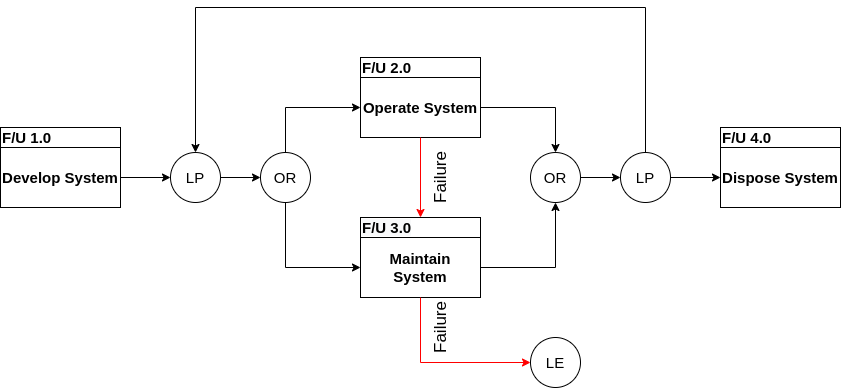
\includegraphics[scale=0.5]{img/L0FF}
	\caption{Level 0 Functional Flow}
	\label{fig:9}
\end{figure}
\noindent
The system will mostly be in the Operate System function seen in \autoref{fig:9}. Once a failure occurs in this state, the system will transition to the Maintain System function. If an unrepairable error occurs, the system will exit the loop and the system will be disposed of.  

\subsection{Level 1}
The level 1 functional flow diagram provides further detail on how the system functions. The blocks from level 0 are expanded to provide more context on that function of the system. The level 1 functional flow of the system is shown in \autoref{fig:10}.
\begin{figure}[H]
	\centering
	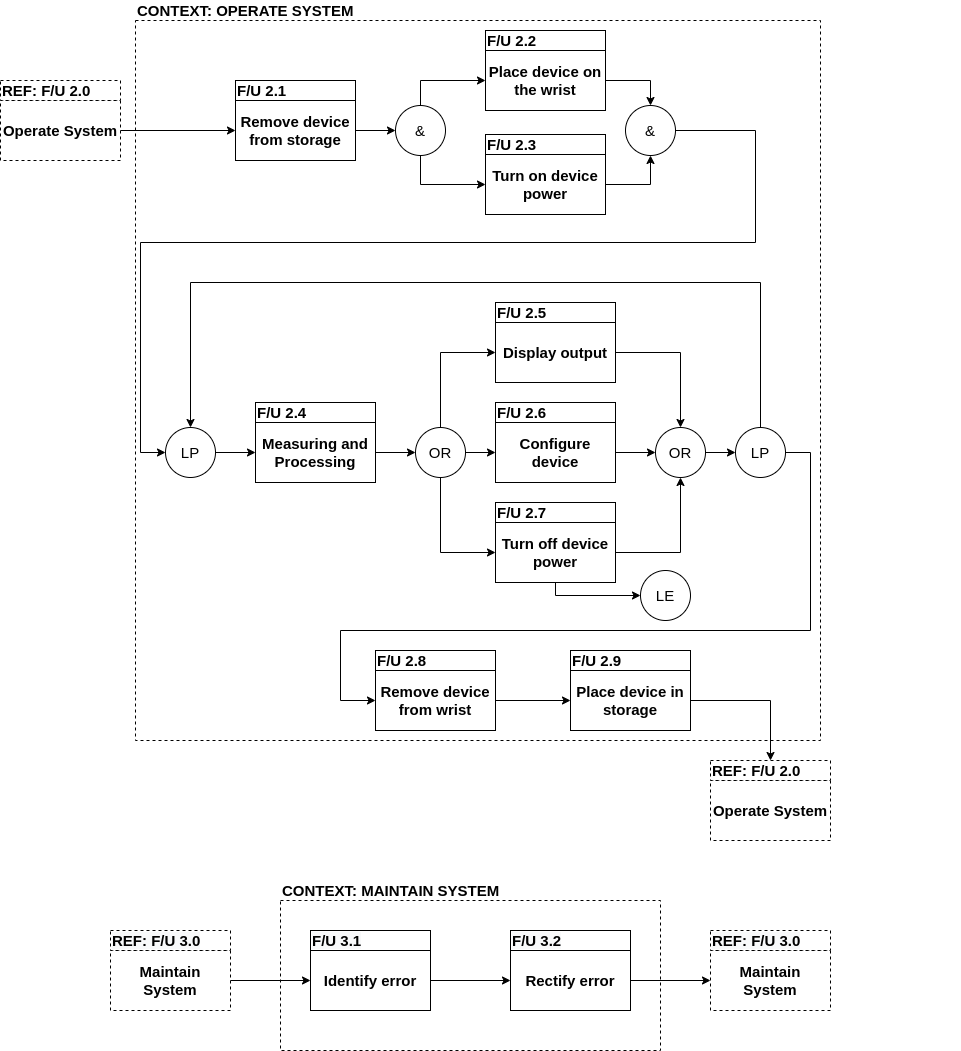
\includegraphics[scale=0.5]{img/L1FF}
	\caption{Level 1 Functional Flow}
	\label{fig:10}
\end{figure}
\noindent
The Operate- and Maintain System functions are expanded in level 1 of the functional flow diagram, and more detailed functions within each are revealed. Some of the blocks in level 1 of the functional flow diagram can be expanded even more. 

\subsection{Level 2}
Level 2 of the functional flow diagram is the in-depth investigation of the blocks from level 1 that can be expanded further. More information on how the system is to function can be seen in level 2 of the functional flow diagram. Blocks from the Operate System context found in \autoref{fig:10}, that can be expanded further are shown in \autoref{fig:11} and \autoref{fig:12}.
\begin{figure}[H]
	\centering
	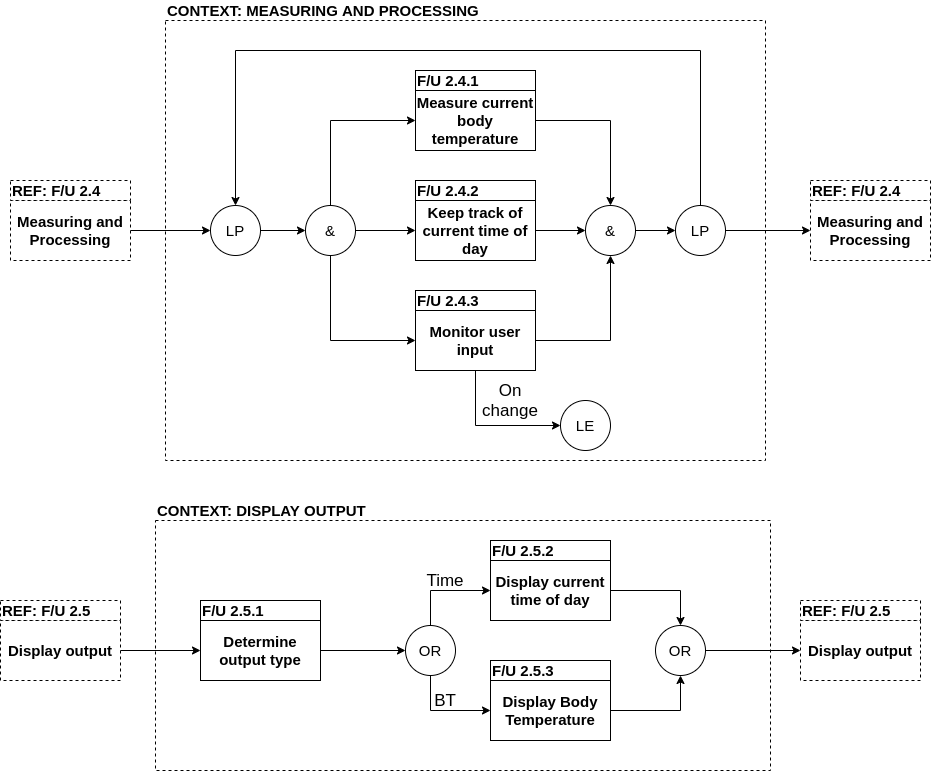
\includegraphics[scale=0.5]{img/L2FF1}
	\caption{Level 2 Functional Flow - Operate System Part 1}
	\label{fig:11}
\end{figure}
\noindent
From \autoref{fig:10} and \autoref{fig:11}, it is clear that the system will mostly be in the Measuring and Processing state where the current body temperature of the user will be measured and general timekeeping will be performed. The system will only go to the next function, which is to display certain information to the user, if prompted. After the system has displayed the requested information, it will return to the Measuring and Processing state. Note, however, that general timekeeping will always be performed by the system, no matter the current function. If the user requests to see the current time of day or current body temperature, the applicable output will be shown.
\begin{figure}[H]
	\centering
	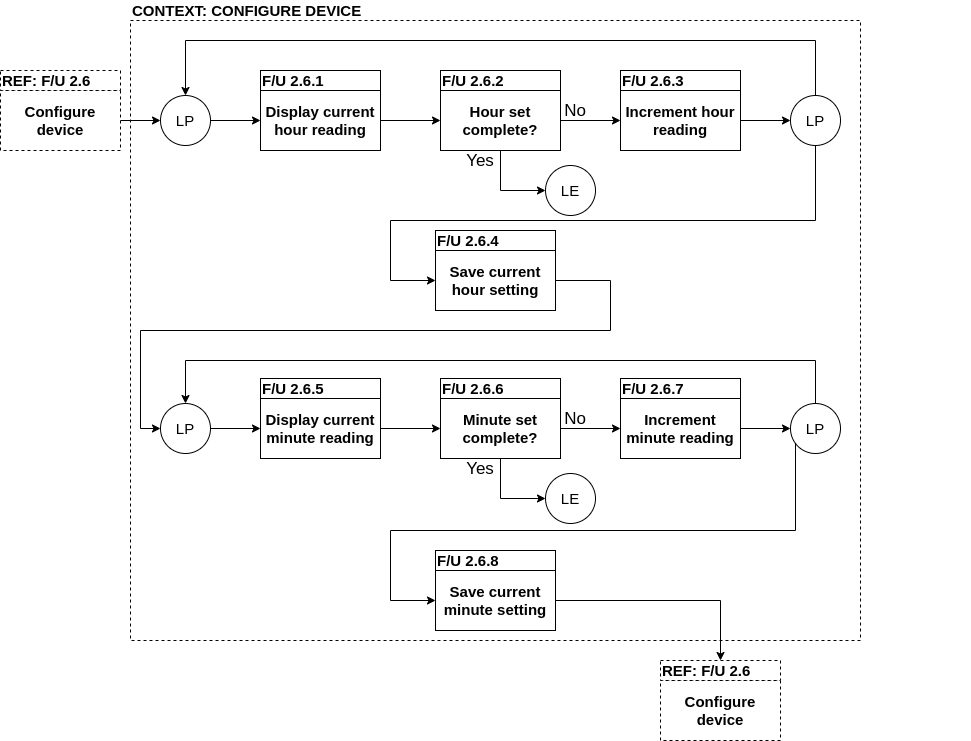
\includegraphics[scale=0.5]{img/L2FF2}
	\caption{Level 2 Functional Flow - Operate System Part 2}
	\label{fig:12}
\end{figure}
\noindent
Once the user requests to configure the device, the current time of day can be set correctly. The process can be seen in \autoref{fig:12}, where the current saved hour reading is shown to the user, this hour reading will be incremented until the user finds it suitable. The hour reading will then be saved. The same process holds for setting the minute reading. 
\\
\\
Blocks from the Maintain System context found in \autoref{fig:10}, that can be expanded further are shown in \autoref{fig:13}.
\begin{figure}[H]
	\centering
	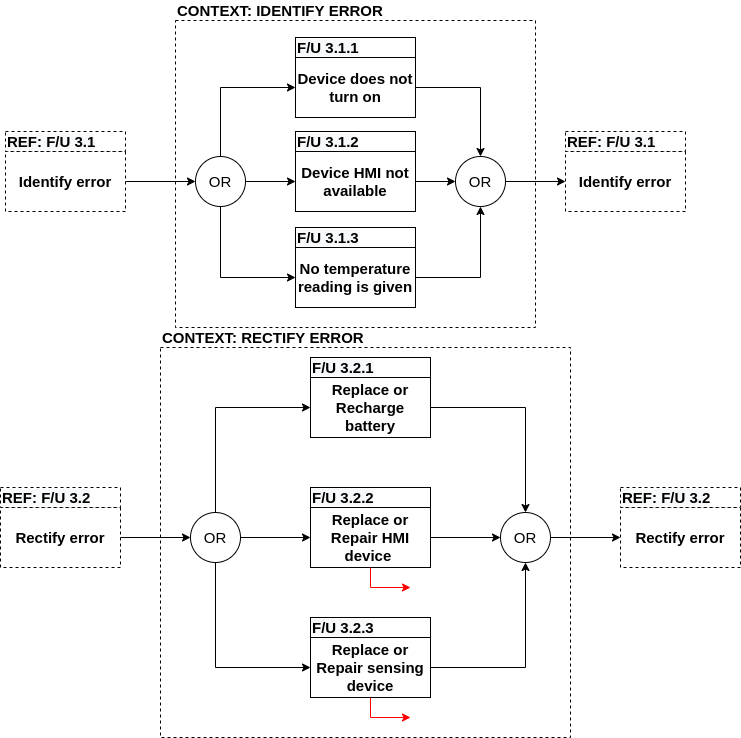
\includegraphics[scale=0.5]{img/L2FF3}
	\caption{Level 2 Functional Flow - Maintain System}
	\label{fig:13}
\end{figure}
\noindent
The Identify error and Rectify error functions from the Maintain System functional diagram are used to find the origin of the error, as well as to rectify the error. If the error is not repairable, the system will transition to the Dispose System state, as mentioned earlier. 

\section{Architectural Synthesis}
Architectural Synthesis is also known as Physical Design and is a process by which the design, that has been captured up to this point in the Functional Analysis, is transformed into something that can be constructed on a concept level. Architectural Synthesis is used to determine what functional elements, or resources, are needed by the system to be able to accomplish the functions mentioned in the previous section. Architectural Synthesis, once again, follows the same level type hierarchy as with the Functional Analysis. In this process, the functional flow elements will be mapped to the physical architecture of the system. 

\subsection{Level 0}
The high level physical architecture of the system is shown in \autoref{fig:14}. At this level, the different objects the system will interact with, denoted as functional units, are seen. 
\begin{figure}[H]
	\centering
	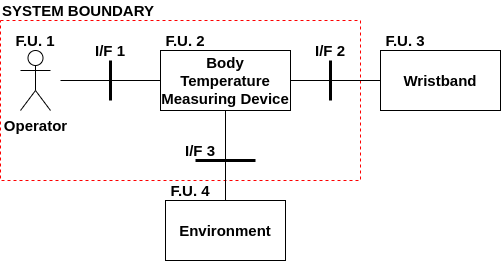
\includegraphics[scale=0.5]{img/L0PA}
	\caption{Level 0 Physical Architecture}
	\label{fig:14}
\end{figure}
\noindent
The system boundary clearly shows the system that will be designed, and the operator or user that will be using the system. Functional Unit 2, which is the Body Temperature Measuring Device is the system of interest, and the Physical Architecture of this unit will be expanded in the level to follow, to show the resources needed to design and construct the system. 

\subsection{Level 1}
The expansion of the Body Temperature Measuring Device from level 0 are shown in \autoref{fig:15}.
\begin{figure}[H]
	\centering
	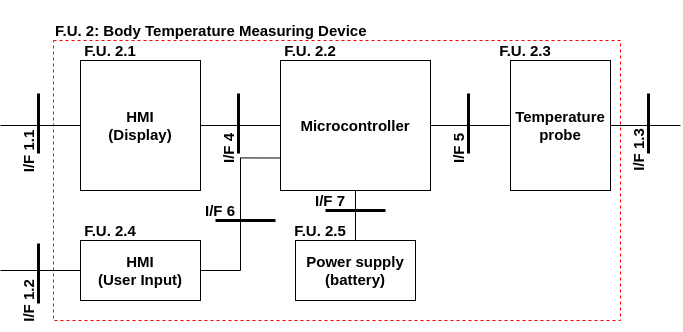
\includegraphics[scale=0.5]{img/L1PA}
	\caption{Level 1 Physical Architecture}
	\label{fig:15}
\end{figure}
\noindent
From \autoref{fig:15} the physical resources needed to implement the system can be seen, as well as how these resources interface with each other and the outside world.
This is the Physical Architecture that will be used in the detailed design of the system, where specific components will be assigned to each resource. 

\section{Resource Allocation}
Resource Allocation matrices are used to test if the conceptual design is valid. A resource allocation matrix compares the available resources to the functions that needs to be performed. Therefore, the functions from the Functional Analysis are compared to the resources from the Architectural Analysis, to see if there is a resource available to perform the specific function, and vice versa. 
\\
\\
The resource allocation matrix that compares the high level functions to the high level resources are shown in \autoref{fig:16}.
\begin{figure}[H]
	\centering
	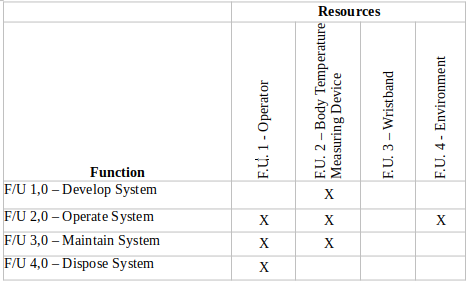
\includegraphics[scale=0.6]{img/RA0}
	\caption{High level Resource Allocation matix}
	\label{fig:16}
\end{figure}
\noindent
The resource allocation matrix that compares the lower level functions to the lower level resources are shown in \autoref{fig:17}.
\begin{figure}[H]
	\centering
	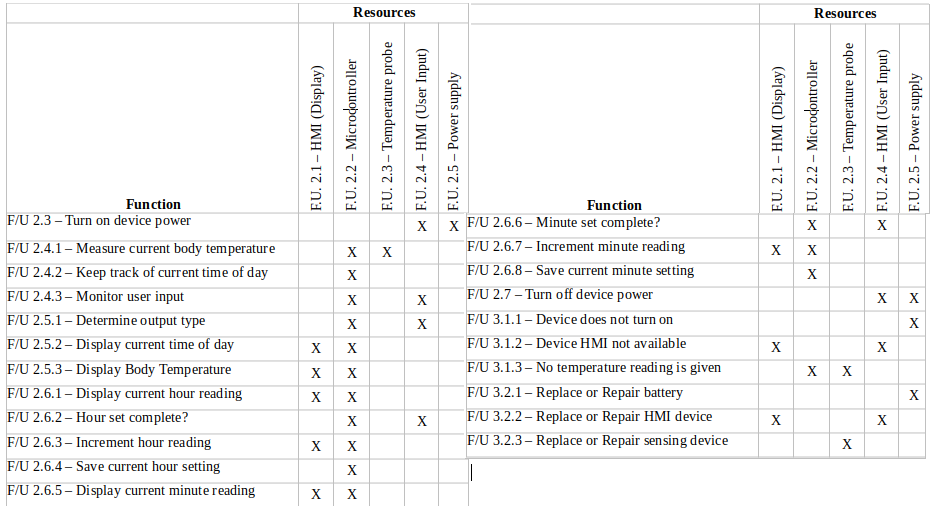
\includegraphics[scale=0.5]{img/RA2}
	\caption{Lower level Resource Allocation matix}
	\label{fig:17}
\end{figure}
\noindent
From the resource allocation matrices it is clear that the concept design is feasible and valid since there are no functions that are not allocated to a resource, and no resources not being used by any functions.

\section{Concluding Remarks}
This section showed the process followed in the concept design of the Medical Wristband Body Temperature Monitor. A Functional Analysis was used to clearly state how the system is to work when fully deployed. After this, an Architectural Synthesis was used to determine the physical architecture of the system, and what resources are available to perform the functions from the Functional Analysis. Finally, Resource Allocation matrices were used for the validation of the concept design. 
	\chapter{Detail Design}\label{Ch4}
In this chapter, the detailed design of the Body Temperature Measuring Wristband will be presented. The detailed design is started with trade-off studies, where Multi-Criteria Decision Matrices (MCDM), together with user-defined utility functions are used to select the specific components required to physically construct the device. The best technique available from the literature study to estimate core body temperature from the temperature of the skin will also be determined. After the selection of components and the measurement technique, the complete circuit of the Body Temperature Measuring Wristband will be given. The design of the embedded firmware will also be presented in this chapter in the form of state machines, as well as firmware flow diagrams.

\section{Trade-off Studies}
In this section, trade-off studies will be performed to select specific components to construct the device. The components that will be selected by the trade-off studies include the temperature probe, the microcontroller, the battery, and the display. Each component will have its own set of criteria, as well as utility functions. In order to determine which component inside the MCDM is best suited, the Weighted Product Method (WPM) algorithm is used. In this algorithm, the utility value of a criterion is raised to the power of the weight of that criterion, and all these weighted scores are then multiplied together. This is done for each alternative component. The formula for WPM is given in \autoref{WPM} \cite{MCDM2020}.
\begin{equation}
    P(A_{K}) = \prod_{j = 1}^{n} (a_{Kj})^{wj}, \;for \;K = 1, 2, 3,....,m.
    \label{WPM}
\end{equation}
\noindent
In this section, the measurement technique will also be selected. This will be done through an analysis and discussion on the advantages and disadvantages of each estimation technique.

\subsection{Microcontroller}
The microcontroller serves as the central processing unit of the body temperature measuring wristband. The microcontroller will be used for communication between the different components, for all the required processing in the process of measuring body temperature, and to distribute power to the components. There are a wide variety of microcontrollers available on the market today, each having its own set of available peripherals, processing speeds, unique features, etc. Therefore, familiar microcontrollers that were available at the time the trade-off studies were conducted, are considered. For the microcontroller of the device, four possibilities were considered:
\begin{itemize}
	\item PIC24FJ64GA004:\\
	The PIC24FJ64GA004 family of microcontrollers are developed by Microchip and is 28/44-pin general-purpose, 16-bit flash microcontrollers. 
	\item PIC24FJ256GA705:\\
	The PIC24FJ256GA705 family of microcontrollers is also developed by Microchip. These are 16-bit general-purpose microcontrollers that have low-power features. 
	\item STM8L15:\\
	The STM8L15 series are developed by STMicroelectronics and are 8-bit ultra-low-power microcontrollers. 
	\item STM32L071KBT6:\\
	The STM32L07 series are also developed by STMicroelectronics and are 32-bit ultra-low-power microcontrollers.
\end{itemize}
\noindent
The evaluation criteria for selecting the microcontroller is:
\begin{itemize}[noitemsep]
	\item Technical Risk
	\item Cost per Unit
	\item Power Consumption
	\item Clock Speed
	\item Lead Time
\end{itemize} 
\noindent
The ability of the designer to correctly implement and interface the specific component with the rest of the circuitry is included in the evaluation criteria as technical risk. Power consumption will play a crucial role in the battery life of the device, and should therefore be kept as low as possible. Since the current drawn by the microcontroller will depend on the connected components, it is difficult to compare power consumption between different microcontrollers. Therefore, the power consumption of the possible microcontrollers is based on the operating current at the lowest clock speed of that microcontroller. This is done so that the microcontrollers can be compared to one another in terms of power consumption, and clock speed. The cost and lead time of the component should be kept as low as possible. Technical Risk is divided into 5 levels and is defined as shown in \autoref{fig:19}. Technical Risk will also be included in the evaluation criteria for the rest of the components and will stay as defined throughout. The utility functions for each criterion are shown in \autoref{fig:21}.
\begin{figure}[H]
	\centering
	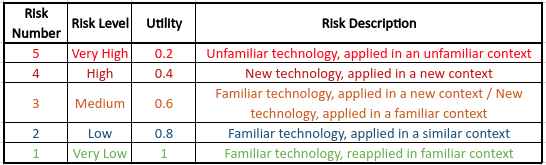
\includegraphics[scale=0.7]{img/Technical Risk}
	\caption{Technical Risk Definition}
	\label{fig:19}
\end{figure}
\begin{figure}[H]
	\centering
	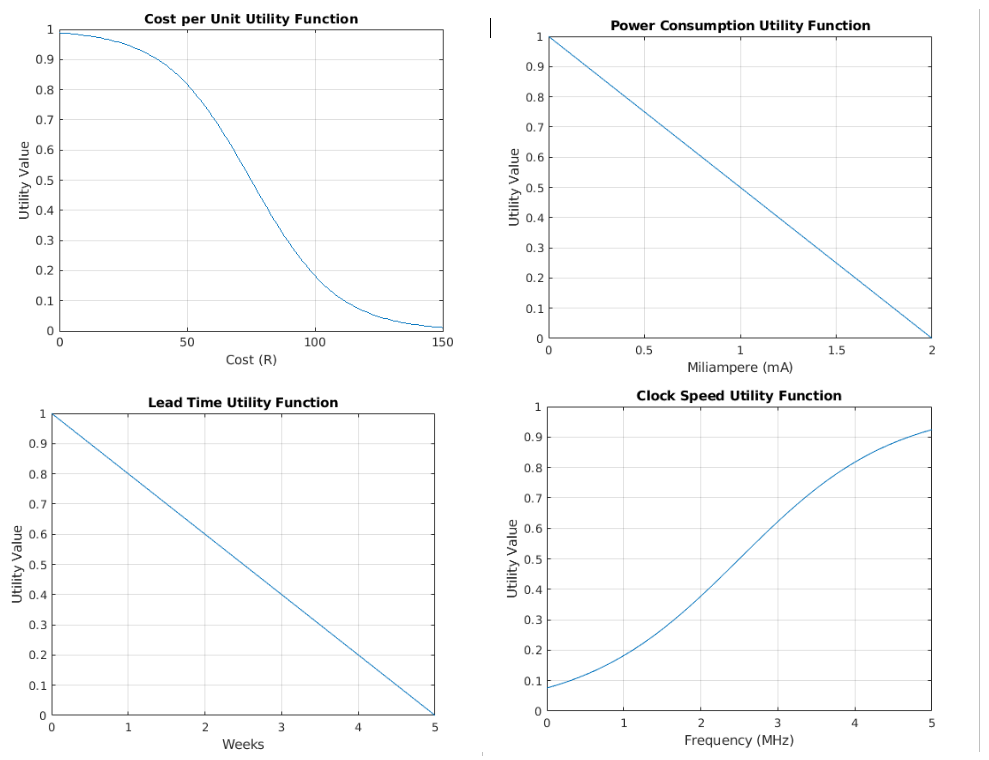
\includegraphics[scale=0.4]{img/M-Util}
	\caption{Microcontroller - Utility Functions}
	\label{fig:21}
\end{figure}
\noindent
The Multi-Criteria Decision Matrices (MCDM) for each microcontroller is shown in \autoref{fig:22}. The weights of the evaluation criteria are chosen according to the importance of the criterion. Power consumption was favoured above clock speed since clock speeds are not as important as power consumption in this energy-efficient application which does require not as much processing. The rest of the evaluation criteria have the same weight as they are of equal importance. All the technical values are obtained from the respective data sheets, the cost is included without tax or shipping to compare the basic microcontroller cost, and the lead time includes shipping. 
\begin{figure}[H]
	\centering
	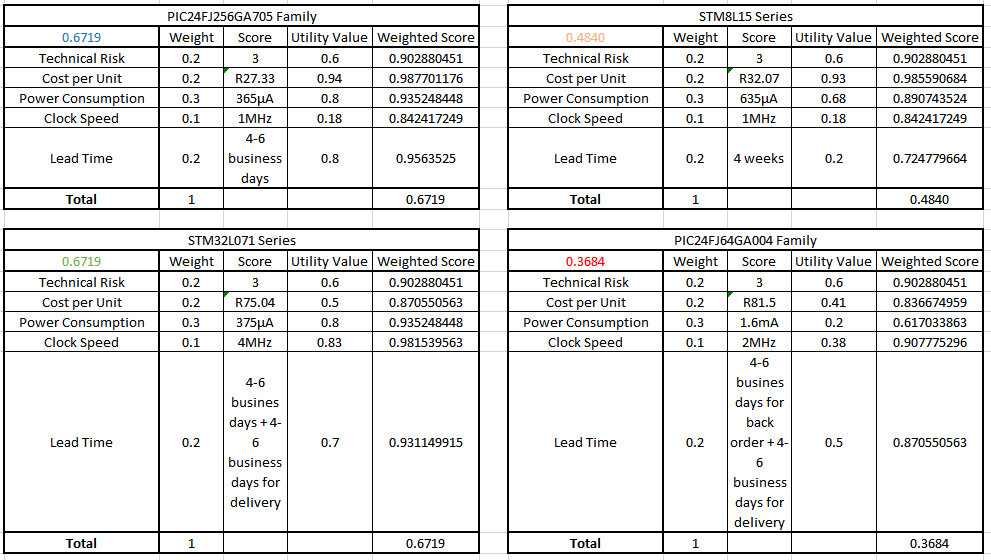
\includegraphics[scale=0.55]{img/M-MCDM}
	\caption{Microcontroller - MCDM}
	\label{fig:22}
\end{figure}
\noindent
From the trade-off study, it is clear that the STM32L071, as well as the PIC24FJ256GA705 series of microcontrollers, are equally suited for this application. The decision is therefore made to use the STM32L071. More specifically, the STM32L071KBT6 of this series will be used. The decision is simply based on preference between STM and PIC microcontrollers.  This microcontroller includes two I2C peripherals, Analog to Digital converters (ADC), Real-Time Clock (RTC) functionality, 128K bytes for program memory, and 20K bytes for RAM. This device has 32 pins, where 25 of them are available for GPIO (General Purpose Input/Output), which will be used for display and input purposes. The STM32L071KBT6 features low power consumption in run mode, and has ultra-low power modes available such as Standby mode (0.29$ \mu $A), Stop mode (0.43$ \mu $A), and Stop mode with RTC (0.86$ \mu $A).

\subsection{Temperature Probe}
The temperature probe will be used to measure the body temperature of the user. For the temperature probe, four possibilities were considered. All of these possibilities have a measurement range that includes the required range for body temperature, and since the chosen microcontroller has many peripherals available, the options may use any possible interface to communicate. The possible temperature probes are:
\begin{itemize}
	\item LM35:\\
	The LM35 is an analog temperature sensor that has an output voltage directly proportional to the measured temperature. 
	\item TMP117:\\
	The TMP117 is a digital temperature sensor integrated circuit (IC) that uses the I2C/SMBus communication protocol.
	\item DS18B20:\\
	The DS18B20 is a digital thermometer that utilises 1-Wire technology for communication with a microprocessor. 
	\item MAX30205:\\
	The MAX30205 is an accurate, low-voltage digital temperature sensor that uses the I2C protocol for communication.
\end{itemize}
\noindent
The evaluation criteria for selecting the temperature probe is:
\begin{itemize}[noitemsep]
	\item Technical Risk.
	\item Measurement Accuracy.
	\item Cost per Unit.
	\item Power Consumption.
	\item Lead Time.
\end{itemize}
\noindent
Since body temperature plays a crucial role in one's health, it must be measured accurately. Therefore, the measurement accuracy of the temperature sensor is included in the criteria. The sensor cost and lead time must be kept as low as possible, as well as the power consumption since the device will be battery operated. The utility functions for each criterion are now given and are shown in \autoref{fig:18}.
\begin{figure}[H]
	\centering
	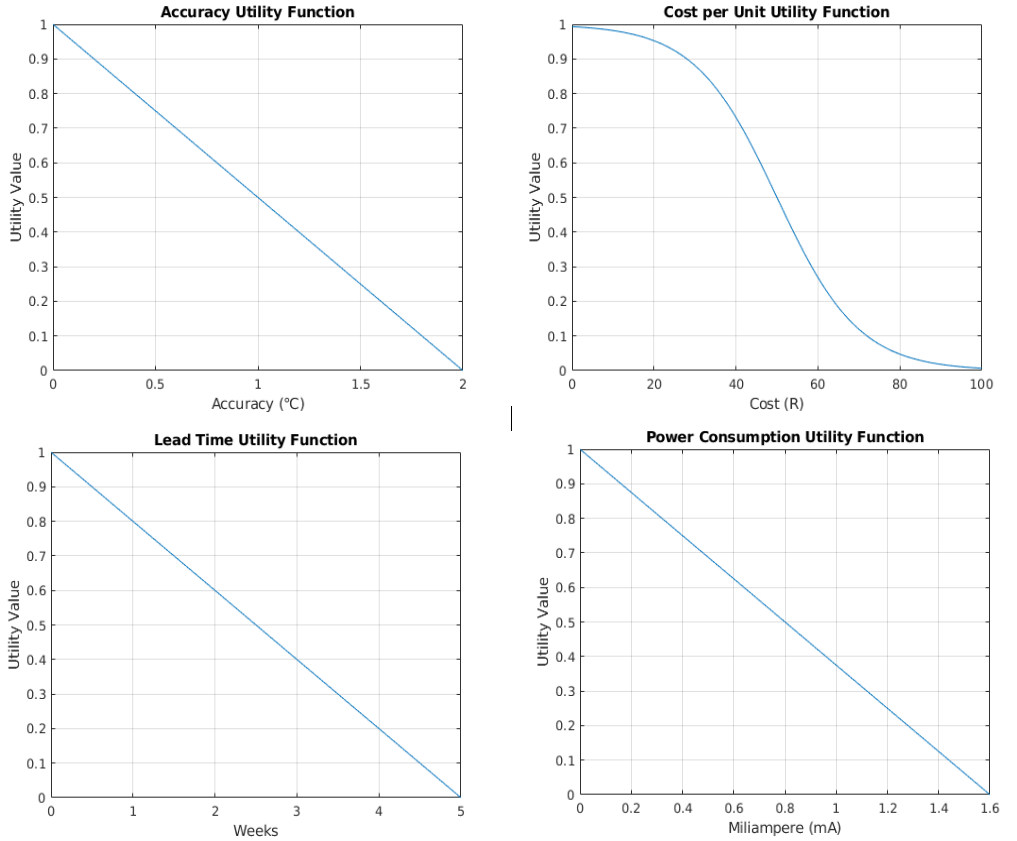
\includegraphics[scale=0.4]{img/T-Util}
	\caption{Temperature Probe - Utility Functions}
	\label{fig:18}
\end{figure}
\noindent
The Multi-Criteria Decision Matrices (MCDM) for each possibility is shown in \autoref{fig:20}. The weights of the evaluation criteria are chosen the same since all the criteria are of equal importance when choosing the temperature probe. All the technical values are obtained from the respective data sheets, the cost is included without tax or shipping to compare the basic sensor cost, and the lead time includes shipping.
\begin{figure}[H]
	\centering
	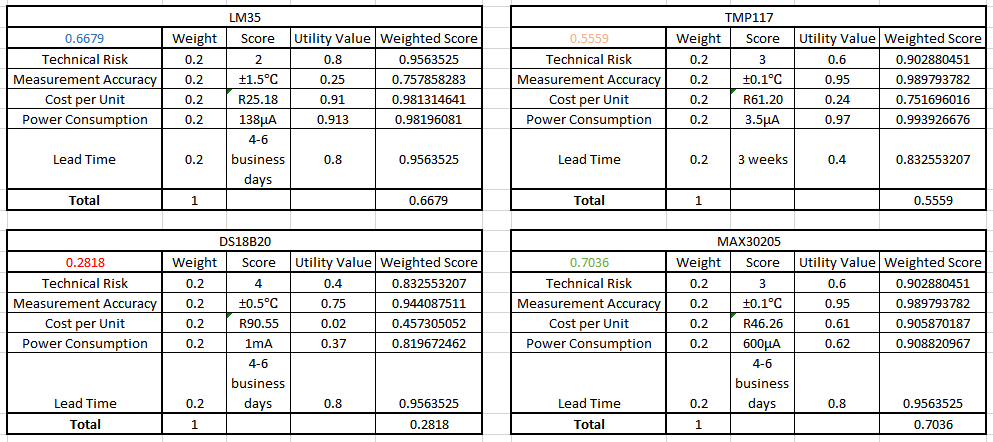
\includegraphics[scale=0.55]{img/T-MCDM}
	\caption{Temperature Probe - MCDM}
	\label{fig:20}
\end{figure}
\noindent
Therefore, the temperature probe that will be used is the MAX30205 digital temperature sensor. 

\subsection{Display}\label{disp}
The display will show the user the measured body temperature, as well as the current time of day. The display will also be used by the user to configure the device. There are various types of displays on the market, ranging from touch screens to LED matrix displays, all coming in a wide variety of sizes. The displays that are considered must be compact and small, energy-efficient, and touch screen are not required. In the case where a driver IC is needed by the display, only the displays that come with the required IC built-in were considered since they do not require any external components or configurations to work properly. For the display of the device, four possibilities were considered:
\begin{itemize}
	\item 0.91 Inch OLED Display Module:\\
	This is an OLED display with 128x32 pixels that comes with an embedded controller that communicates via the I2C interface. 
	\item 4 Digit 7-Segment LED Display:\\
	This is a display consisting of four standard 7-segment displays that are connected together in one package.  
	\item Midas 0.49in White Passive Matrix OLED Display:\\
	This is a 64x32 resolution OLED display that has a white-on-black appearance, that also comes with an embedded controller that communicates via I2C.
	\item RS PRO TFT LCD Colour Display:\\
	This display is a full-colour TFT LCD module with a normally white backlight. The screen has a 160x80 resolution and the display communicates via a 3- or 4-wire serial peripheral interface.
\end{itemize}
\noindent
The evaluation criteria for selecting the display is:
\begin{itemize}[noitemsep]
	\item Technical Risk.
	\item Size of the Module.
	\item Cost per Unit.
	\item Power Consumption.
	\item Lead Time.
\end{itemize}
\noindent
The size of the display will play a crucial role in the overall size of the final device and should be kept as small, yet as legible as possible since the device will be in the form of a wristband. The device will be battery operated, and the power consumption by the display should be as low as possible in order to provide longer battery life. The cost and lead time should, once again, be as low as possible. The utility functions for each criterion are shown in \autoref{fig:25}.
\begin{figure}[H]
	\centering
	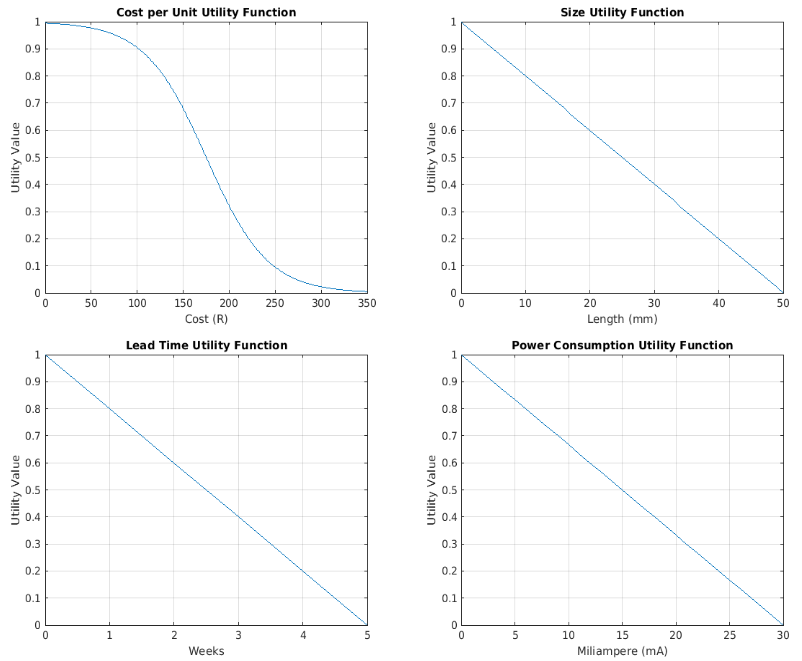
\includegraphics[scale=0.5]{img/D-Util}
	\caption{Display - Utility Functions}
	\label{fig:25}
\end{figure}
\noindent
The Multi-Criteria Decision Matrices (MCDM) for each possibility is shown in \autoref{fig:26}. All the technical values are obtained from the respective data sheets, the cost is included without tax or shipping to compare the basic sensor cost, and the lead time includes shipping. The weights of the evaluation criteria are chosen the same since all the criteria are equally important. Although the size of the screen plays a very important role, it cannot have a higher weight than the other criteria since they are of equal importance.
\begin{figure}[H]
	\centering
	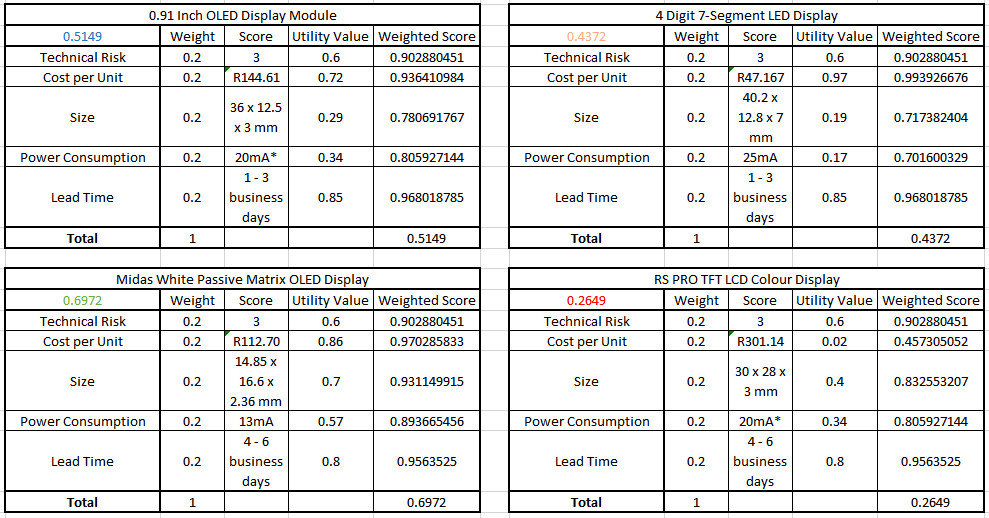
\includegraphics[scale=0.55]{img/D-MCDM}
	\caption{Display - MCDM}
	\label{fig:26}
\end{figure}
\noindent
From the trade-off study, it is clear that the White Passive Matrix OLED Display from Midas will be best suited for the body temperature measuring device. As mentioned previously, this display has a 64x32 resolution and has the SSD1306 controller built-in on the display module, and communicates via the I2C interface. 


\subsection{Battery} 
The battery will provide power to the microcontroller, as well as the other components of the device. For the battery, two different possibilities that are easily accessible were considered:
\begin{itemize}
	\item RS PRO LIR2032:\\
	This is a rechargeable button battery with a chemical composition of Lithium-ion.
	\item RS PRO Lithium Polymer battery:\\
	This is a Li-Polymer rechargeable battery that has a low self-discharge and comes pre-wired with bare wire terminals.
	\item Panasonic CR2032 Button battery:\\
	This is a non-rechargeable coin cell battery that have a low self-discharge rate.
\end{itemize}
\noindent
The evaluation criteria for selecting the battery is:
\begin{itemize}[noitemsep]
	\item Technical Risk
	\item Cost per Unit
	\item Size
	\item Capacity
	\item Lead Time
\end{itemize}
\noindent
Since the developed device will be in the form of a wristband, the size of the product must be small, to provide maximum comfort. In order to compare the button batteries to the battery that has a square shape, only the length of each will be considered. The capacity of the battery will determine how long the body temperature wristband will last, and therefore, the higher the capacity, the better. As previously, the cost and lead time should be as low as possible. The utility functions for each criterion for the battery are shown in \autoref{fig:23}, and the Technical Risks are defined once again as in \autoref{fig:19}.
\begin{figure}[H]
	\centering
	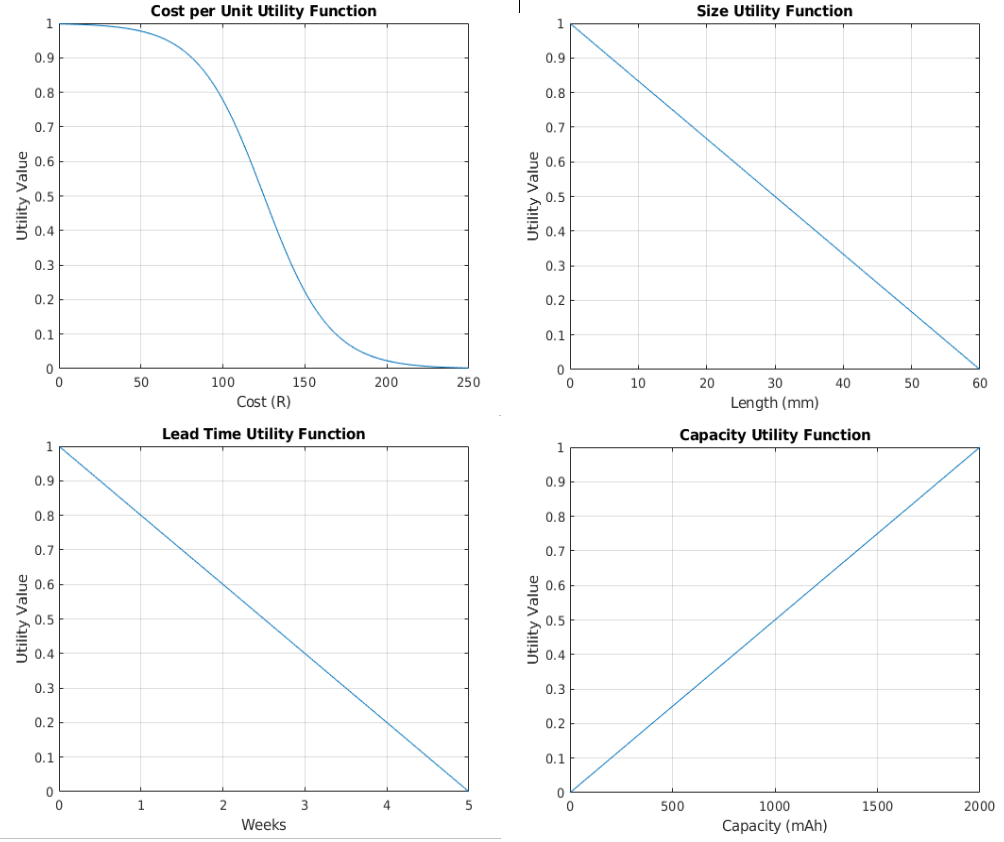
\includegraphics[scale=0.4]{img/B-Util}
	\caption{Battery - Utility Functions}
	\label{fig:23}
\end{figure}
\noindent
The Multi-Criteria Decision Matrices (MCDM) for each battery is shown in \autoref{fig:24}. Capacity and size are favoured in terms of the evaluation weight above the other criteria since they are of most importance in choosing the battery. Technical Risk is given a lower weight as the use of batteries is straightforward, although battery management and recharging may be more complex. Lead time is also given a lower weight since batteries are relatively easily accessible. The cost is included without tax or shipping to compare the basic battery cost, the lead time includes shipping, and all the technical values are obtained from the respective datasheets.
\begin{figure}[H]
	\centering
	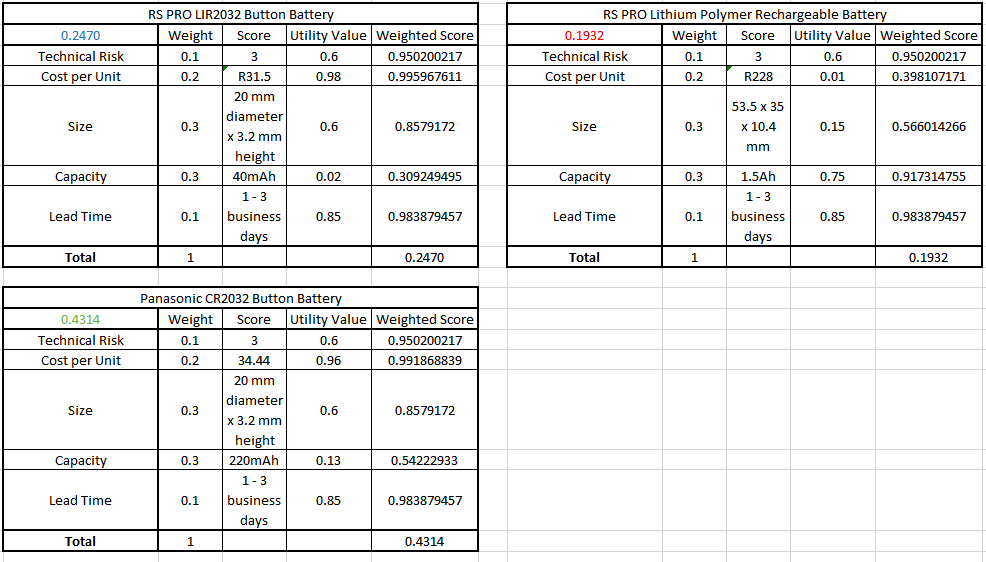
\includegraphics[scale=0.55]{img/B-MCDM}
	\caption{Battery - MCDM}
	\label{fig:24}
\end{figure}
\noindent
Therefore, the battery that will be used is the Panasonic CR2032 Button battery. This battery is non-rechargeable as mentioned previously, and it has a nominal voltage of 3.0V. The nominal voltage of the battery will be sufficient to power the microcontroller, which has a supply voltage range of 1.65V to 3.6V. This nominal voltage is also sufficient to power the temperature probe which has a 2.7V to 3.3V supply voltage rating, and the display, which can be powered from 2V to 5V. The big advantage of this battery is that no extra recharging circuitry, which will consume a lot of space, is needed. This type of battery is also commonly available in grocery stores, garages, etc. making it easily accessible when it must be replaced. 

\subsection{Measurement Technique}\label{technique}
In \autoref{Sec2_4} of this report, several non-invasive techniques to measure core body temperature from skin temperature were introduced. To determine which of these methods will be best suited to implement on the Body Temperature Monitor, a less analytical method than previous, are followed. The advantages, as well as disadvantages of each technique, are compared to one another, to determine which technique is best suited. The advantages and disadvantages of each technique are summarised below.
\begin{itemize}
    \item Zero-heat-flow:\\
    Advantage(s): Estimates Core Body Temperature accurately.\\
    Disadvantage(s):  Heater element consumes a lot of power. Extra components are needed (Heater, Thermal insulator, 2x Thermistors).
    
    \item Dual-heat-flux:\\
    Advantage(s): Estimates Core Body Temperature accurately, while using less energy than the zero-heat-flow method.\\
    Disadvantage(s): Four temperature probes are needed. Long measurement time. Systems based on this method are relatively large.
    
    \item Thermal Equivalent Circuit:\\
    Advantage(s): Estimates Core Body Temperature accurately, and takes ambient temperature into consideration. \\
    Disadvantage(s): Requires the thermal resistance of the body, which may differ from person to person. This method also requires that the probe is wrapped in a highly thermally conductive material.
    
    \item Statistical Estimation:\\
    Advantage(s): Estimates Core Body Temperature accurately, whilst taking ambient conditions and different skin types into consideration in the development of the statistical model. \\
    Disadvantage(s): This technique will require a lot of data or samples to build an accurate and reliable statistical modal.
\end{itemize}
\noindent
All of the techniques mentioned above estimates Core Body Temperature relatively accurately, and ambient conditions are accounted for within each technique. Therefore, to determine which technique is best, the disadvantages of each technique will be compared to each other. 
\\
\\
The device must be energy efficient, hence it can be concluded that the zero-heat-flow method is not the best-suited technique for this application, since the heater element used in this technique will consume a lot of power. The dual-heat-flux may result in a device that is relatively large in size, and also more expensive since four temperature probes are required. The thermal equivalent circuit model requires the thermal resistance of the body. The thermal resistance may differ from person to person, and from skin to skin, which may result in inaccurate temperature readings for some people. Therefore, the best technique for this application is a statistical estimation. Although this technique requires a lot of data to build an accurate statistical model, no extra components are needed, the size of the device can be kept as small as possible, and it will be the most energy-efficient measurement technique to use for this application. Since the technique is based on statistical models, which can be improved by gathering more data, the accuracy of the device can be improved even after it is physically constructed.

\section{Physical Architecture}
In this section the updated physical architecture of the Medical Wristband Body Temperature Monitor is shown. The components from the trade-off studies in the previous section are added to the diagram, as well as some interfaces between the components. The detailed physical architecture of the device is shown in \autoref{fig:27}.
\begin{figure}[H]
	\centering
	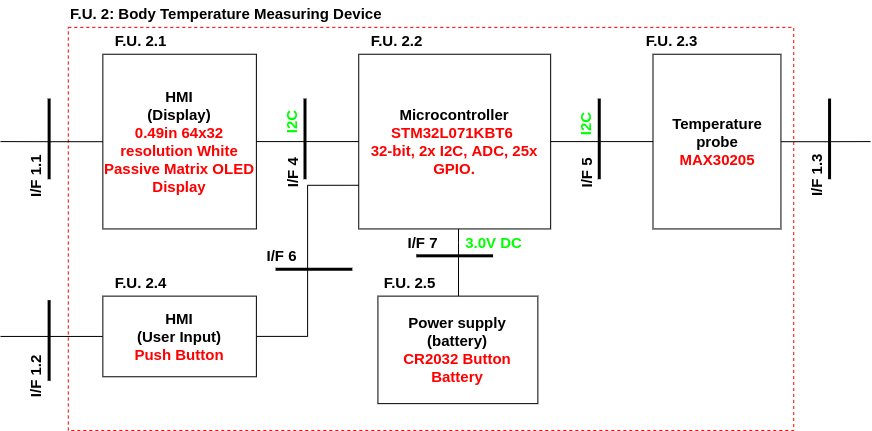
\includegraphics[scale=0.5]{img/Detail_PA}
	\caption{Detailed Physical Architecture}
	\label{fig:27}
\end{figure}


\section{Schematics}
This section will show the schematics for the Body Temperature Measuring device. The schematic of the device will be broken down into sub-systems to aid legibility, however, the full schematic can be found in \autoref{FSchematic}. The sub-systems for the Body Temperature Measuring device are as follow:
\begin{itemize}[noitemsep]
	\item The Microcontroller and all relevant components.
	\item The Temperature sensor and all relevant components.
	\item The user input buttons.
	\item The Power supply unit.
	\item External component connectors.
\end{itemize}

\subsection{Microcontroller}
This section will show the schematic for the microcontroller of the device. All the components related to the microcontroller, such as decoupling capacitors, resistors, etc. are also shown in the schematic. The microcontroller and relevant circuits can be referred to as the processing unit of the device. The schematic for the processing unit of the device is shown in \autoref{fig:28}. 
\begin{figure}[H]
	\centering
	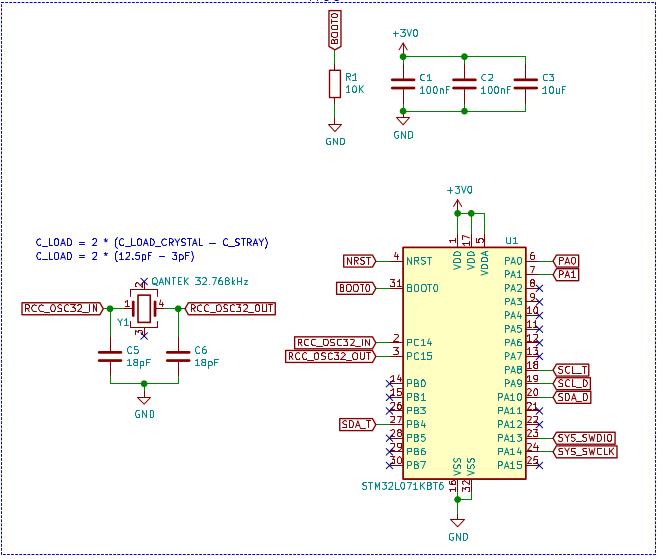
\includegraphics[scale=0.6]{img/Schematic_MCU}
	\caption{Schematic: Microcontroller}
	\label{fig:28}
\end{figure}
\noindent
From \autoref{fig:28} all the connections to and from the microcontroller can be seen as the connections are labelled. These labels show the physical connections to all the other components of the device, as two labels with the same value are connected.  
\\
\\
\autoref{fig:28} shows that there are three decoupling capacitors for the microcontroller. From the datasheet of the STM32L071KBT6, ST recommends that for every $ V_{DD} $ and $ V_{SS} $ pair of the microcontroller, a $ 100 nF $ capacitor is needed. They also recommend that in addition to the $ N \times 100 nF $ capacitors, one $ 10 \mu F $ capacitor is needed. It can be seen that the $ BOOT0 $ pin of the microcontroller is pulled to ground via a resistor. This is done to hold the logic level near 0V on this pin. The $ BOOT0 $ pin must be at the defined low logic level (ground) to select the main flash memory as the boot space of the microcontroller. 
\\
\\
A low-speed external (LSE) crystal oscillator is also connected to the microcontroller. This crystal oscillator will be used as the frequency source of the RTC. The microcontroller features a low-speed internal RC oscillator that may be used for this purpose, but internal low-speed clocks tend to have a low accuracy, which is not ideal for time-keeping purposes. The decision is therefore made to add a $ 32.768 kHz $ external crystal oscillator to the microcontroller. This value of $ 32.768 kHz $ is commonly used as the frequency in RTC applications since it is a power of 2 ($ 2^{15} $) value and one can get a precise 1 second period ($ 1 Hz $) by using a 15 stage binary counter. Sometimes, a feed resistor is needed between the oscillator and the microcontroller. A feed resistor limits the amount of drive going to and from the crystal ensuring that the crystal waveform is not distorted. However, ST strongly recommends not to add an external resistor between the oscillator pins of the microcontroller. Two load capacitors can be seen at the crystal oscillator. The values of the load capacitors are calculated by using the following formula:
\begin{equation}
C_{load} = 2 \times (C_{crystal} - C_{stray})
\end{equation}
\noindent
Where $ C_{crystal} $ is the load capacitance of the crystal which is found in the datasheet as $ 12.5 pF $, and $ C_{stray} $ is the stray capacitance of the PCB which is assumed as $ 3 pF $. Therefore, $ 19 pF $ is the calculated value of the load capacitors, and the nearest commercial capacitor value that could be found is $ 18 pF $.

\subsection{Temperature Sensor}
This section will show the schematic for the temperature sensor of the device. The schematic for the MAX30205 temperature sensor is shown in \autoref{fig:29}.
\begin{figure}[H]
	\centering
	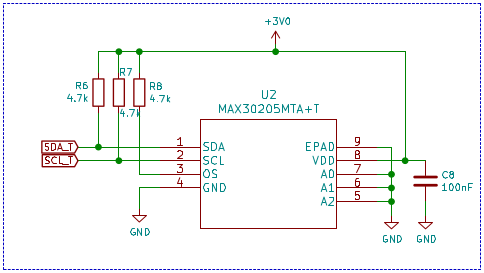
\includegraphics[scale=0.6]{img/Schematic_Temp}
	\caption{Schematic: Temperature sensor}
	\label{fig:29}
\end{figure}
\noindent
From \autoref{fig:29} it can be seen that three pull-up resistors are needed, one for the Serial Clock Line (SCL), one for Serial Data Line (SDA), and one for Over-temperature Shut-down (OS). It can also be seen that a $ 100 nF $ capacitor is needed between $ V_{DD} $ and ground. This is obtained from an application circuit in the MAX30205 datasheet. This temperature sensor communicates via I2C and in \autoref{fig:29} it shows that the MAX30205 are connected to pins 18 (SCL) and 27 (SDA) of the microcontroller. Since $ A0 $, $ A1 $, and $ A2 $ are all connected to ground, the slave address in hex of the temperature sensor is 90h.
 
\subsection{User Input buttons}
The user input buttons will be used to wake the device from standby mode, as well as to change what is being displayed by the device. The device will also be configured by one of the input buttons. The schematics for the two input buttons are shown in \autoref{fig:30}.
\begin{figure}[H]
	\centering
	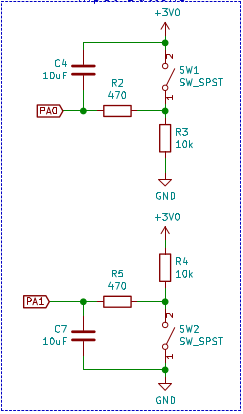
\includegraphics[scale=0.7]{img/Schematic_Button}
	\caption{Schematic: Input Buttons}
	\label{fig:30}
\end{figure}
\noindent
From \autoref{fig:30} it can be seen that one of the input buttons of the device has an active-high configuration, whilst the other input button has an active-low configuration. The active-high button is used to wake the microcontroller from standby or low-power mode. This needs to be an active-high configuration since the device will only wake on the rising edge of any of the three wake-up (WKUP) pins. Pin 6 (PA0) is used in this case to wake the device. The active-low button is used as an input button so that the user can change what is being displayed by the device, and also set the current time and date, etc. The reason an active-low configuration is used to capture the input of the user is to ensure that it is functional if and only if an intentional logic state is applied. Therefore, ambiguous floating input conditions are avoided in the process. The input button is connected to pin 7 (PA1) of the microcontroller.
\\
\\
It can also be seen that both the buttons have a de-bouncing circuit. This is to deal with the mechanical bounce of the switch contacts after they are hit together (button was pressed) since most microcontrollers will interpret this bouncing action as separate hits of the button.

\subsection{Power Supply}
This section will show the power supply of the body temperature measuring device. The device will be battery operated as mentioned previously. The power supply of the device is shown in \autoref{fig:31}.
\begin{figure}[H]
	\centering
	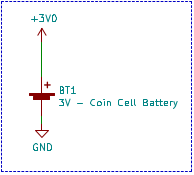
\includegraphics[scale=0.7]{img/Schematic_Battery}
	\caption{Schematic: Power Supply}
	\label{fig:31}
\end{figure}
\noindent
From \autoref{fig:31} it can be seen that the power supply of the device is just a single coin cell battery. No voltage regulator is required since all of the components of the device have an input voltage range that includes the 3V being delivered by the battery. 

\subsection{External Component Connectors}
The display, as well as the flash programmer, must connect to the device externally. This section will show the schematics for the external component connectors.
\subsubsection{Display Connector}
Although the display is part of the body temperature measuring device, it will be connected externally to the device since the display is in the form of a module. The connection between the display and the main circuit of the body temperature device will be made through header pins. Therefore, to ensure communication between the microcontroller and the display, it must be accommodated for in the schematic. The display that will be used (determined in \autoref{disp}) has the following pinout as obtained from the datasheet:
\begin{table}[H]
	\centering
	\caption{\textit{Display pinout}}
	\label{tab:4}
		\begin{tabular}{|c|c|}
		\hline
		\textbf{Pin} & \textbf{Symbol}\\
		\hline
		\hline
		1 & GND\\
		\hline
		2 & VCC\\
		\hline
		3 & SCL\\
		\hline
		4 & SDA\\
		\hline
	\end{tabular}
\end{table}
\noindent
The schematic for the display connector is shown in \autoref{fig:32}. The display communicates to the microcontroller via the I2C interface, and it will be connected to pins 19 (SCL) and 20 (SDA) of the microcontroller via the display connector..
\begin{figure}[H]
	\centering
	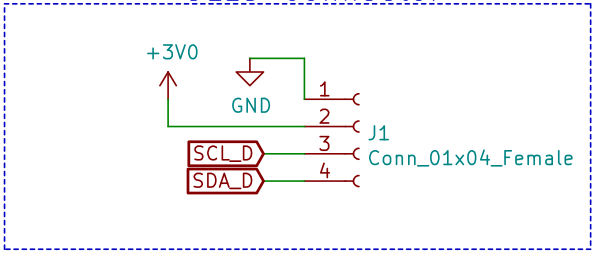
\includegraphics[scale=0.6]{img/Schematic_Disp}
	\caption{Schematic: Display Connector}
	\label{fig:32}
\end{figure}
\subsubsection{Flash Connector}
The Flash connector or from now on SWD (Serial Wire Debug) connector, will be used to flash program code onto the microcontroller. An ST-LINK/V2-1 will be used to flash the code onto the device. The ST-LINK that will be used has the following pinout, which shows the required connections to the microcontroller in order to flash program code on to the device:
\begin{table}[H]
	\centering
	\caption{\textit{SWD Connector}}
	\label{tab:5}
	\begin{tabular}{|c|c|c|}
		\hline
		\textbf{Pin} & \textbf{Symbol} & \textbf{Designation}\\
		\hline
		\hline
		1 & VDD\_Target & VDD from application\\
		\hline
		2 & SWCLK & SWD clock\\
		\hline
		3 & GND & Ground\\
		\hline
		4 & SWDIO & SWD data input/output\\
		\hline
		5 & NRST & RESET of target STM32\\
		\hline
	\end{tabular}
\end{table}
\noindent
The schematic for the SWD connector is shown in \autoref{fig:33}. The connector allows communication between the microcontroller and the ST-LINK, and is connected to pins 4 (NRST), 23 (SYS\_SWDIO) and 24 (SYS\_SWCLK) of the microcontroller.
\begin{figure}[H]
	\centering
	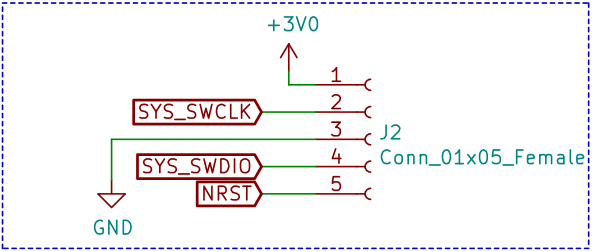
\includegraphics[scale=0.6]{img/Schematic_SWD}
	\caption{Schematic: SWD Connector}
	\label{fig:33}
\end{figure}

\section{Firmware}
The firmware that will be flashed onto the microcontroller that will be controlling the behavior of the device will be discussed in this section. The firmware is developed in the embedded C programming language. Rather than to show the developed code in this section, the finite state machine of the software will be shown to indicate the different states, and how to transition from one state to the other. This section will also show flow diagrams of the firmware that is created for the device. The state diagrams will show the different states of the device, where the flow diagrams will show the steps taken by the software during execution and the logical flow of the software.

\subsection{Finite State Machine}
A high-level state machine of the device is shown in \autoref{FSM}. In this figure, it can be seen that upon startup of the device, it will display the measured temperature of the user. The user can then press the button for less than one second to see the current time of day and press the button again for less than one second, to see the date. If the user then presses the button once again for less than one second, the temperature will be displayed again. This cycle just mentioned is the Normal Mode in which the device is operating. The current display mode will keep displaying (Self-Transition) until one transition condition is met. If this self-transition cycled for more than 5 seconds, the device will go into Standby Mode.
\\
\\
If the user wants to change the current time or date, he/she must navigate to either the time- or the date display mode and then press the button between 1.5 and 3 seconds to enter Settings Mode. In settings mode the user will cycle through all possible settings, starting at setting the hour and ending by setting the year. A short press of the button (<=1 sec) will increment the current setting, and a long press (1.5 < sec <= 3) will transition to the next setting.
\begin{figure}[H]
	\centering
	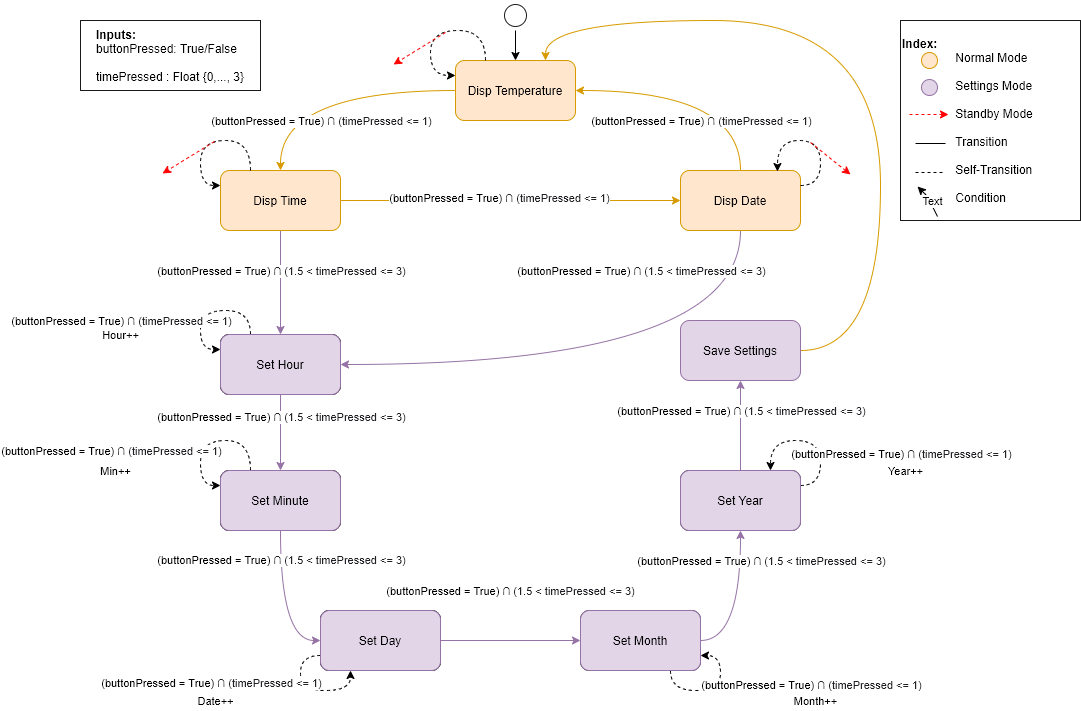
\includegraphics[scale=0.4]{img/FSM.png}
	\caption{Finite State Machine}
	\label{FSM}
\end{figure}

\subsection{Flow Diagrams}
From the FSM of the device, it is clear that there are 8 possible states that the device can be in. These states are now numbered to be referred to in the flow diagrams, and the numbering is as follow:
\begin{table}[H]
	\centering
	\caption{\textit{States of the device}}
	\label{tab:7}
	\begin{tabular}{|c|c|c|}
		\hline
		\textbf{State} & \textbf{Description} & \textbf{Mode}\\
		\hline
		\hline
		0 & Measure and Display Temperature & Normal\\
		\hline
		1 & Display Time & Normal\\
		\hline
		2 & Display Date & Normal\\
		\hline
		3 & Set Hour & Settings\\
		\hline
		4 & Set Minute & Settings\\
		\hline
		5 & Set Day & Settings\\
		\hline
		6 & Set Month & Settings\\
		\hline
		7 & Set Year & Settings\\
		\hline
	\end{tabular}
\end{table}
\noindent
The main flow diagram of the firmware is shown in \autoref{Flow-Diag1}
\begin{figure}[H]
	\centering
	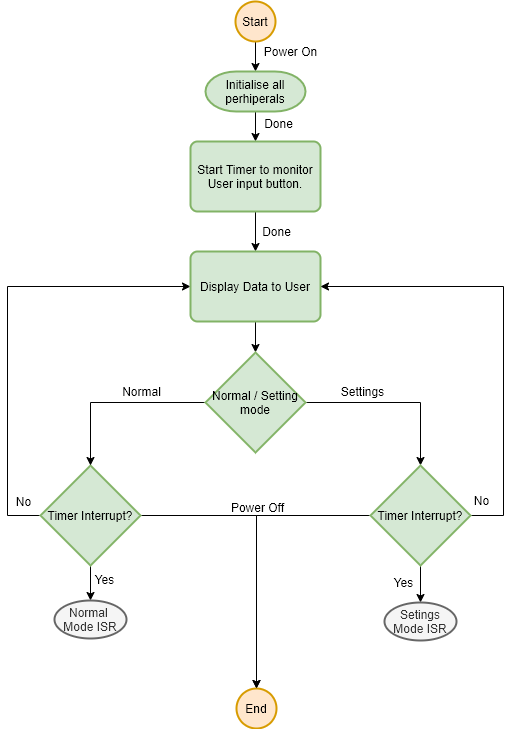
\includegraphics[scale=0.5]{img/Flow-Diag1.png}
	\caption{Main Flow Diagram}
	\label{Flow-Diag1}
\end{figure}
\noindent
From the main flow diagram of the firmware, it can be seen that when the device power-up, all the configured peripherals will be initialised. These peripherals include both I2C channels, GPIO pins, the RTC as well as all the timers used. After the peripherals are initialised, the timer used to monitor the user input button (polling) is started. Then, the requested data will be displayed to the user. On startup, the displayed data will be the user's temperature since this is the default state as seen in \autoref{FSM}. The default mode is therefore the Normal Mode. The firmware will then continuously monitor if the input button is pressed by the user. The status of the button will be monitored inside the respective mode's Interrupt Service Routine (ISR). This is demonstrated in \autoref{Flow-Diag2} and \autoref{Flow-Diag3}.
\\
\\
\autoref{Flow-Diag2} shows the flow diagram for the ISR for when in Normal Mode.
\begin{figure}[H]
	\centering
	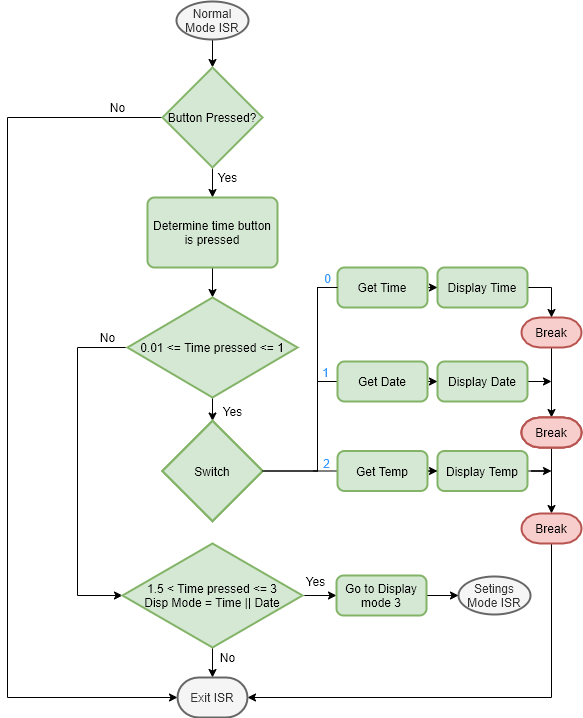
\includegraphics[scale=0.5]{img/Flow-Diag2.png}
	\caption{Normal Mode ISR}
	\label{Flow-Diag2}
\end{figure}
\noindent
From the flow diagram of the Normal Mode ISR, it can be seen that when an interrupt is triggered from \autoref{Flow-Diag1}, the firmware will determine if the button is pressed. If the button is not pressed, the firmware will return to the "Display Data to User" block of the main flow diagram. If, however, the user presses the button, the firmware will count how long the button is pressed. As mentioned earlier, if the button is pressed less than one second ( <= 1 sec), what is being displayed to the user will cycle through displaying temperature, displaying the time, and displaying the date. The blue number in the switch case refers to the current state of the device, and the corresponding green block shows to which state or display mode the device will transition into. 
\\
\\
If the button is pressed longer ( 1.5 < sec <= 3) and the current state is either to display time or date, the device will transition to Settings Mode. Settings Mode has its own ISR, and the flow diagram can be seen in \autoref{Flow-Diag3}.
\begin{figure}[H]
	\centering
	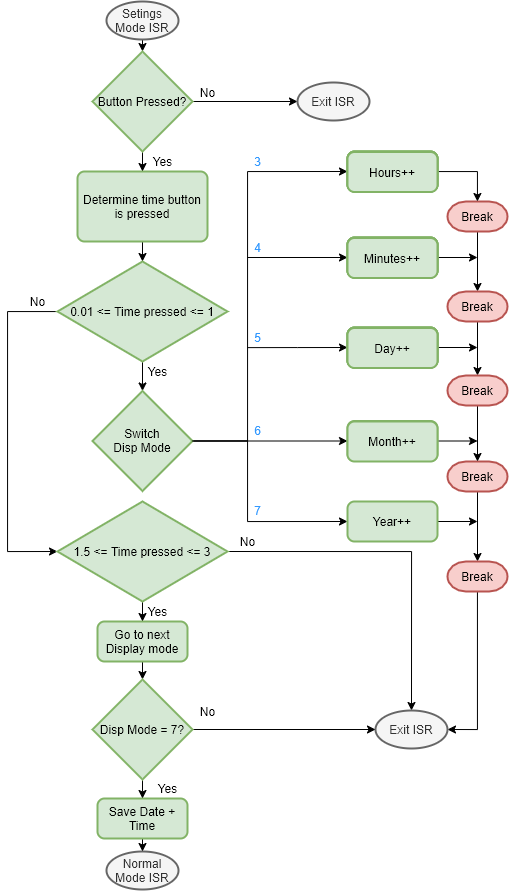
\includegraphics[scale=0.5]{img/Flow-Diag3.png}
	\caption{Settings Mode ISR}
	\label{Flow-Diag3}
\end{figure}
\noindent
Just as with the ISR for the Normal Mode, the firmware will determine if the button is pressed, and for how long the button is pressed. Once again, if the button is not pressed by the user, the firmware will return to the main flow diagram. If the button is pressed for less than one second ( <= 1 sec), the current setting that is being changed will be incremented. Therefore, if the current state is 3, the hours will be incremented, and if the current state is 4, the hours will be incremented, etc. The blue number in the switch case refers to the current state of the device. If the button is then pressed for a longer time ( 1.5 < sec <= 3), the current state will be incremented to allow the user to set the hours, minutes, date, month and year. If then the last state is reached, the newly set date and time will be saved by the firmware, and the firmware will return to Normal Mode.

\section{Concluding Remarks}
This chapter focused on the detailed design of the Body Temperature Monitoring Wristband. Components were selected by utilising Multi-Criteria Decision Matrices (MCDM) using the Weighted Product Method (WPM). Only the microcontroller, the temperature probe, battery, and display were selected in this way. The selected components can be summarised as in \autoref{tab:6}:
\begin{table}[H]
	\centering
	\caption{\textit{Component Summary}}
	\label{tab:6}
	\begin{tabular}{|c|c|}
		\hline
		\textbf{Category} & \textbf{Component} \\
		\hline
		\hline
		Microcontroller & STM32L071KBT6 \\
		\hline
		Temperature Probe & MAX30205\\
		\hline
		Display & Midas White Passive Matrix OLED Display \\
		\hline
		Battery & CR2032 Button Battery \\
		\hline
	\end{tabular}
\end{table}
\noindent
Statistical estimation was determined as the technique that will be used to estimate core body temperature from the temperature of the skin. After the component and measurement technique selections, the full schematic diagram of the designed device was given with a few design choices explained. Lastly, the firmware that will be flashed on the device was designed by means of a state machine that show the different possible states of the device and how to transition from one state to another. Firmware flow diagrams were also given to show the exact flow of the firmware, as well as the steps taken during software execution. 
	\chapter{Implementation and Testing}\label{Ch5}
In this chapter, the detailed design of the Body Temperature Measuring Wristband from the previous chapter will be implemented and tested. This will be done by firstly designing a Printed Circuit Board (PCB) in CAD software. After the PCB is designed and physically constructed, it will be populated with all the required components. Then the testing phase will begin, where each aspect of the Body Temperature Measuring Wristband will be tested to confirm the expected working of the device.

\section{Implementation}
In this section, the layout and design of the PCB of the Body Temperature Monitoring Wristband will be given. Since the size of the device must be kept as small as possible, the overall footprint of the PCB must also be kept to a minimum. 2D models of the PCB will be given, as well as a 3D model to see how the designed PCB will look like. This section will also show the manufactured and populated PCB of the device. 

\subsection{Printed Circuit Board Design}
The device will have a two-layer PCB, allowing components to either be on the top or the bottom layer. The temperature sensor and related components are on the bottom layer to ensure that it is always in contact with the skin of the user, whilst the other components such as the microcontroller, display, power source, etc. are on the top layer. The software representation of the top 2D view, the bottom 2D view, as well as the combined 2D view of the PCB is shown in \autoref{PCB-Top}, \autoref{PCB-Bottom} and \autoref{PCB-Comb} respectively.
\begin{figure}[H]
	\centering
	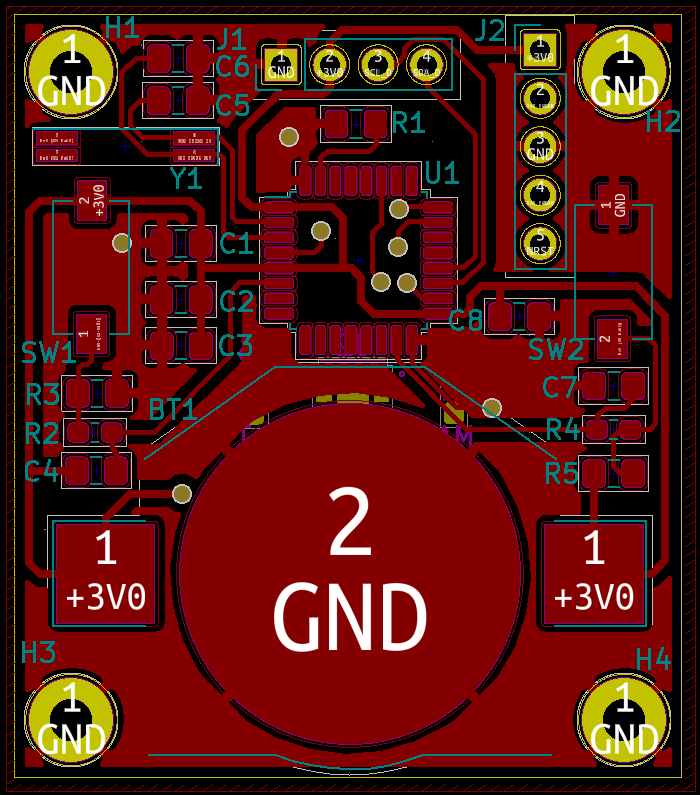
\includegraphics[scale=0.4]{img/PCB-Top.PNG}
	\caption{Software PCB: 2D Top View}
	\label{PCB-Top}
\end{figure}
\begin{figure}[H]
	\centering
	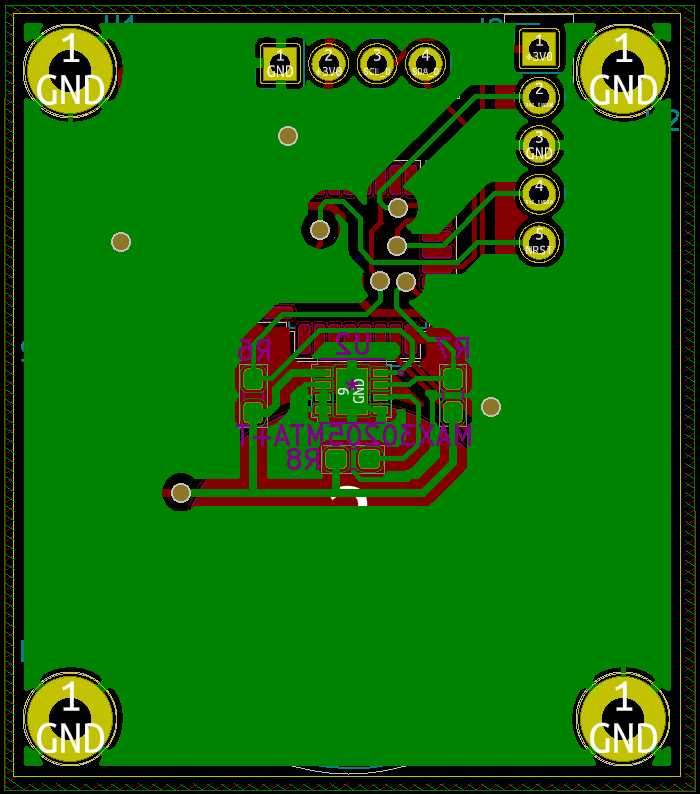
\includegraphics[scale=0.4]{img/PCB-Bottom.PNG}
	\caption{Software PCB: 2D Bottom View}
	\label{PCB-Bottom}
\end{figure}
\begin{figure}[H]
	\centering
	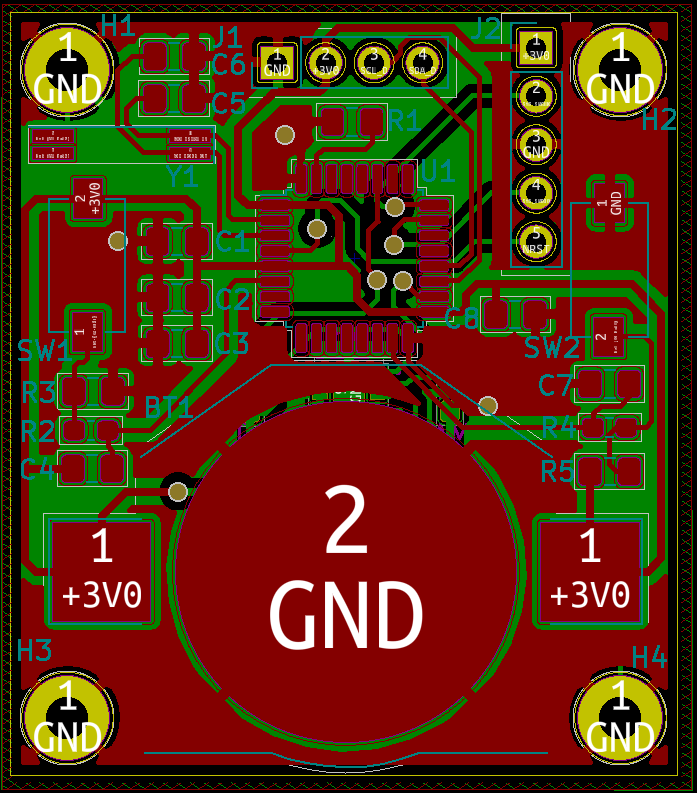
\includegraphics[scale=0.4]{img/PCB-Comp.PNG}
	\caption{Software PCB: 2D Combined View}
	\label{PCB-Comb}
\end{figure}
\noindent
In order to get a better understanding on how the PCB will look like, a 3D rendering of the PCB with all the components populated is shown in \autoref{PCB-3D}.
\begin{figure}[H]
	\centering
	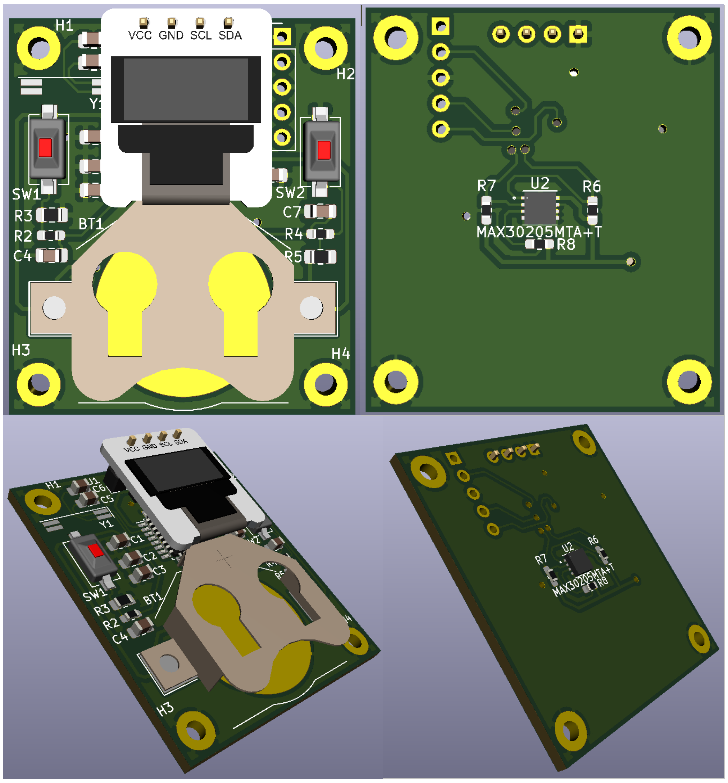
\includegraphics[scale=0.8]{img/PCB-3D.PNG}
	\caption{Software PCB: 3D View}
	\label{PCB-3D}
\end{figure}
\noindent
The dimensions of the designed PCB are shown in \autoref{PCB-Dim}. From this figure, as well as the previous figures showing the PCB layout, it can be seen that the overall footprint of the PCB was kept as small as possible by spacing the components as compactly as the design tolerances would allow. Surface mount components were used where possible and available since through-hole components generally have a larger footprint than that of surface mount components.
\begin{figure}[H]
	\centering
	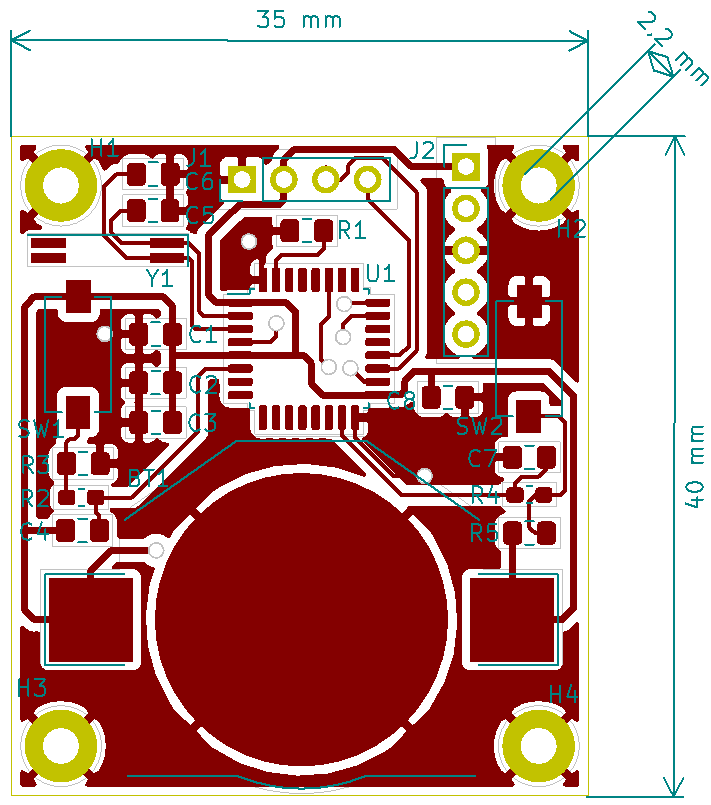
\includegraphics[scale=0.4]{img/PCB-Dim.PNG}
	\caption{PCB: Dimensions}
	\label{PCB-Dim}
\end{figure}

\subsection{Manufactured Prototype Printed Circuit Board}
The manufactured prototype PCB that is populated with the components is shown in this subsection. The top view of the manufactured PCB is shown in \autoref{MPCB-Top} and the bottom view of the PCB is shown in \autoref{MPCB-Bottom}. The testing of the device will be discussed in a later section of this chapter.
\begin{figure}[H]
	\centering
	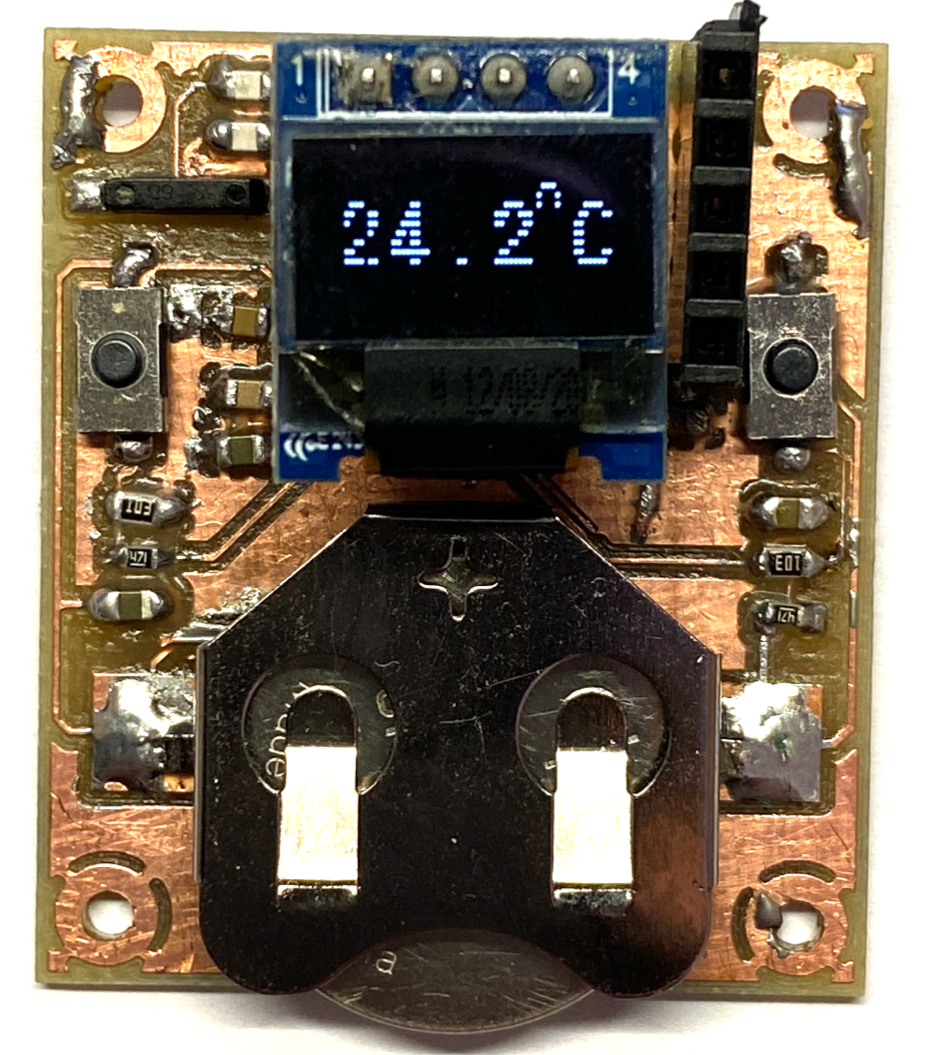
\includegraphics[scale=0.3]{img/MPCB-Top.PNG}
	\caption{Manufactured PCB: Top View}
	\label{MPCB-Top}
\end{figure}
\begin{figure}[H]
	\centering
	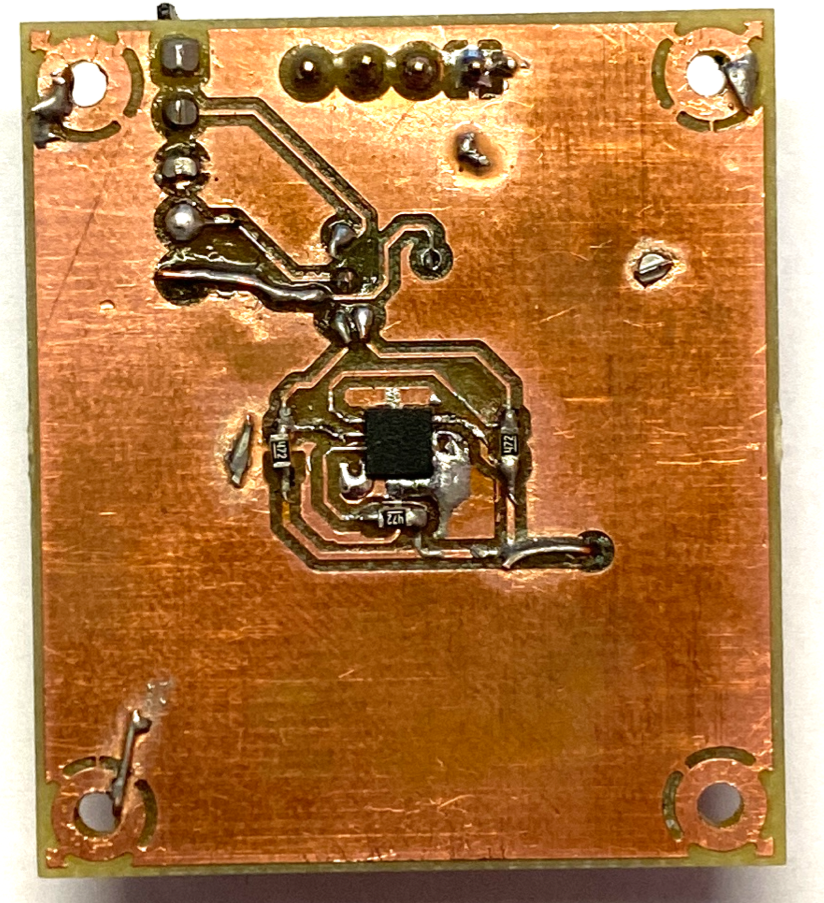
\includegraphics[scale=0.3]{img/MPCB-Bottom.PNG}
	\caption{Manufactured PCB: Bottom View}
	\label{MPCB-Bottom}
\end{figure}

\subsection{Statistical Estimation Model}\label{estm}
In this section, the technique to estimate core body temperature from skin temperature will be discussed. In \autoref{technique} of this report, the statistical estimation is selected as the best technique for this purpose. The method to build the statistical model is explained in \autoref{stat} of this report. The statistical model that will be used for this device is based on that developed by Kwak et al. \cite{Kwak2019} in 2019. In this study, a large amount of data is collected by measuring the skin temperature, the ambient temperature, and the corresponding body temperature to use as a reference in the statistical model. Kwak et al. made the statistic model by collecting data from four students (two men and two women) from May to August 2018 \cite{Kwak2019}. Kwak et al. then derived the relationship between body temperature and skin temperature using the collected data and the method that is described in \autoref{stat} of this report. 
\\
\\
The derived relationship is \cite{Kwak2019}:
\begin{equation}
    Y = 0.109X + 33.07
    \label{estimate}
\end{equation}
\noindent
This relationship are implemented in the firmware to estimate the user's body temperature ($ Y $) from the skin temperature measured by the device ($ X $).

\section{Testing and Results}
In this section, the developed Body Temperature Monitor is tested and results are shown where applicable. 

\subsection{Flash Connector}
The goal of this test is to determine if the STM32 microcontroller of the device can communicate with the ST-LINK/V2-1. This is done in order to verify that the program code can be successfully flashed onto the device. STM developed a tool named STM32 ST-LINK Utility specifically for this reason. This tool will be used to test if communication is possible. \autoref{STLink} shows the result of this test. 
\begin{figure}[H]
	\centering
	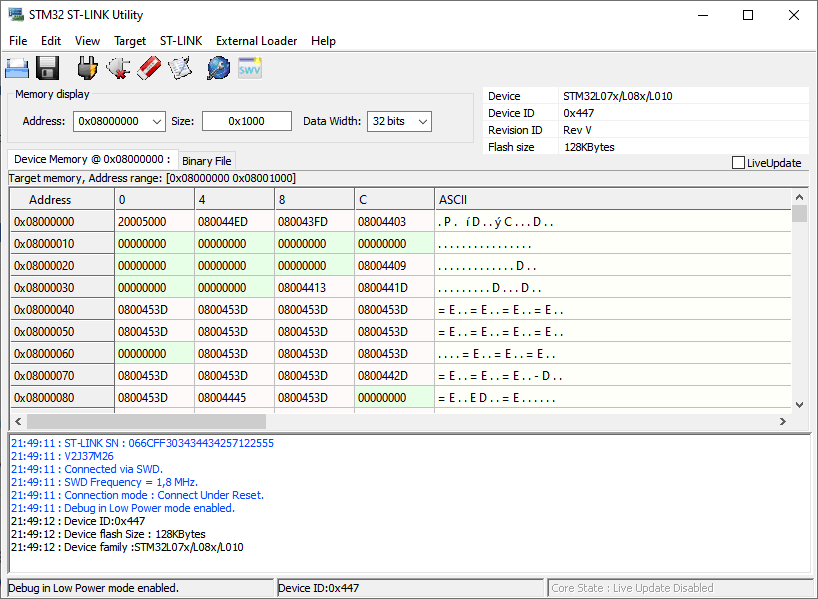
\includegraphics[scale=0.7]{img/STLink.png}
	\caption{STM32 Flash Connection Test}
	\label{STLink}
\end{figure}
\noindent
From the figure above it can be seen that the ST-LINK can successfully connect to the microcontroller of the device through SWD. 

\subsection{Measurement of Skin Temperature}
In this subsection, the accuracy of the measured skin temperature will be determined. Hence, it will be determined how accurate the Body Temperature Measuring device can measure skin temperature compared to a known reference measurement. During this experiment, \autoref{estimate} is not applied in the firmware of the device, resulting in just the measured skin temperature being displayed by the device. To measure the reference temperature (the correct temperature), a Type K thermocouple strapped to the wrist of the user, is used. The Body Temperature Measuring device is then also strapped to the wrist of the user, next to the thermocouple. The error between the two measurements is taken as the absolute difference between the reference temperature and the measured temperature by the device, and the accuracy of the measurement is determined with \autoref{acc}.
\begin{equation}
    Accuracy = 100\% - ((\frac{|Measured - Reference|}{Reference})*100)
    \label{acc}
\end{equation}
\noindent
A few measurements are made during the course of one day, with the method as explained above. The full data-set of the measurements can be found in \autoref{Exp-Data}. \autoref{skin-temp} shows a graph of the reference temperatures versus the measured temperatures. 
\begin{figure}[H]
	\centering
	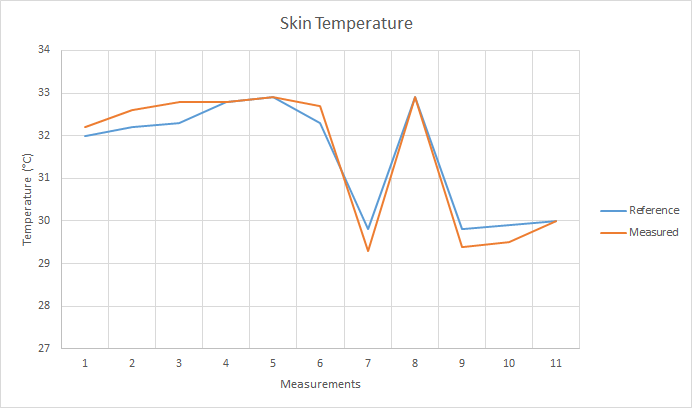
\includegraphics[scale=0.7]{img/Skin-Temp.png}
	\caption{Measurement of Skin Temperature}
	\label{skin-temp}
\end{figure}
\noindent
From \autoref{skin-temp} it can be seen that the temperature measured by the Body Temperature Measuring device varies as the skin temperature varies. The largest absolute difference between the reference temperature and the measured temperature is determined as $ 0.5^{\circ} C $, and the smallest absolute difference is $ 0^{\circ} C $. These absolute errors then relates to a $ 98.32 \%$ measurement accuracy at least, and $ 100 \% $ measurement accuracy at best, for the measurement of skin temperature. 

\subsection{Measurement of Body Temperature}\label{MBT}
In this subsection, the accuracy of the measured body temperature will be determined. Hence, the accuracy by which body temperature gets estimated will be determined. During this experiment, \autoref{estimate} is applied in the firmware of the device, in order for the device to estimate the body temperature of the user by measuring the skin temperature. The reference body temperature of the user is measured with a digital thermometer that is placed under the tongue of the user. The Body Temperature Measuring device is then strapped to the wrist of the user. Once again, the error between the two measurements is taken as the absolute difference between the reference temperature and the estimated body temperature obtained from the device. The accuracy of the measurements is determined with \autoref{acc}.
\\
\\
The measurements are made during the course of two days, at random intervals, with the method as explained above. The number of measurements that were made are 22, and the full data-set of the measurements can be found in \autoref{Exp-Data}. The digital thermometer that are used as a reference measures and displays the body temperature of the user within one minute. When the digital thermometer indicates that its measurement is complete, the temperature that is given by the Body Temperature Measuring device is noted and both these results are added to the data-set. \autoref{body-temp} shows a graph of the reference body temperatures versus the estimated body temperatures.
\begin{figure}[H]
	\centering
	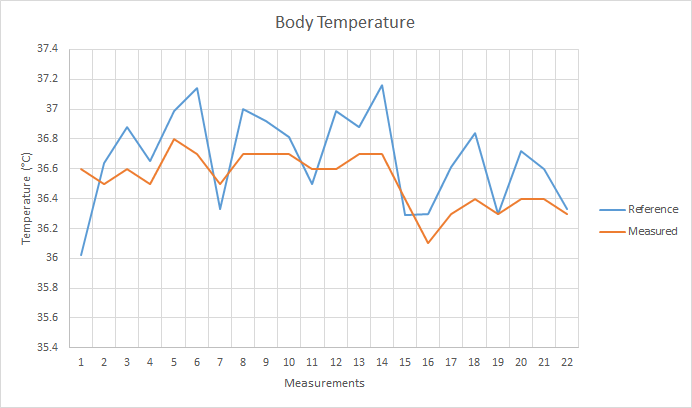
\includegraphics[scale=0.7]{img/Body-Temp.png}
	\caption{Measurement of Body Temperature}
	\label{body-temp}
\end{figure}
\noindent
From \autoref{body-temp} it can be seen that the estimated body temperature relatively varies as the body temperature of the user varies. The largest absolute difference between the reference body temperature and the estimated body temperature is determined as $ 0.58^{\circ} C $. The smallest absolute difference is determined as $ 0^{\circ} C $. These absolute errors then relate to a $ 98.39 \%$ measurement accuracy at least, and $ 100 \% $ measurement accuracy at best, for the estimation of body temperature from the temperature of the skin.

\subsection{Current Consumption of Device}
In this subsection, the current consumption of the device will be determined. This is done to estimate the battery life of the device. The ammeter is series connected into the circuit of the device, and the following measurements are obtained:
\begin{table}[H]
	\centering
	\caption{\textit{Run Mode Current Consumption}}
	\label{tab:8}
	\begin{tabular}{|c|c|}
		\hline
		\textbf{State} &  \textbf{Consumption (mA)} \\
		\hline
		\hline
		Display Temp & 4.49 \\
		\hline
		Display Time & 4.95 \\
		\hline
		Display Date & 5.02\\
		\hline
		Set Hour & 4.72\\
		\hline
		Set Min & 4.71\\
		\hline
		Set Date & 4.68 \\
		\hline
		Set Month & 4.90 \\
		\hline
		Set Year & 5.05 \\
		\hline
		\textbf{AVG} & \textbf{4.815}\\
		\hline
	\end{tabular}
\end{table}
\begin{table}[H]
	\centering
	\caption{\textit{Standby Mode Current Consumption}}
	\label{tab:9}
	\begin{tabular}{|c|c|}
		\hline
		\textbf{State} &  \textbf{Consumption (mA)} \\
		\hline
		\hline
		Standby & 0.01\\
		\hline
	\end{tabular}
\end{table}
\noindent
To estimate the battery life of the device, it is assumed that the user uses the device two times every hour, for 10 seconds. The rest of the time the device will be in standby mode to preserve battery life. An online battery life calculator is used to estimate the battery life. The online calculator is called: Battery Life Calculator for Projects with Sleep Mode, and this calculator includes a 15\% deterioration rate to account for some discharge \cite{Calc2021}. The following were entered into the online calculator:
\begin{itemize}[noitemsep]
    \item Capacity rating of battery (mAh) = 220
    \item Current consumption of device during sleep (mA) = 0.01
    \item Current consumption of device during wake (mA) = 4.815
    \item Number of wakeups per hour (3600 = always ON) = 2
    \item Duration of wake time (ms) = 10000
\end{itemize}
\noindent
The online calculator estimates the battery life of the device as 212.34 days, or 0.58 years, based on the assumptions above. 

\section{Concluding Remarks}
This chapter focused on the implementation and testing of the Body Temperature Monitoring Wristband. Firstly the PCB design of both the top and bottom layers was given, together with a 3D rendered view of the populated PCB. The dimensions of the designed PCB were also given. After this, the manufactured prototype PCB was shown, both the top layer and the bottom layer. In this chapter, the statistical estimation model was also given. The model was based on that developed by Kwak et al. \cite{Kwak2019}, and the relationship between skin temperature and body temperature is given.
\\
\\
After the implementation process was completed, testing began. The communication between the ST-LINK and the STM32 microcontroller of the device was tested, and it was found that communication between the ST-LINK and the microcontroller is possible. This means that firmware can be flashed onto the microcontroller. Next, the accuracy of the device was tested, and the results are shown in \autoref{results}.
\begin{table}[H]
	\centering
	\caption{\textit{Testing Summary}}
	\label{results}
	\begin{tabular}{|c|c|c|}
		\hline
		\textbf{} & \textbf{Skin Temperature} & \textbf{Body Temperature} \\
		\hline
		\hline
		Largest absolute error ($ ^{\circ} C $) & 0.5 & 0.58\\
		\hline
		Smallest absolute error ($ ^{\circ} C $) & 0 & 0\\
		\hline
		Lowest measurement accuracy (\%) & 98.32 & 98.39\\
		\hline
		Highest measurement accuracy (\%) & 100 & 100\\
		\hline
	\end{tabular}
\end{table}
\noindent
The current consumption of the device was also measured, to estimate the battery life of the device. If the device is used two times every hour, for 10 seconds, the estimated battery life of the device is 212.34 days or 0.58 years.


	\chapter{Conclusions and Recommendations}\label{Ch6}
The final chapter concludes the report. The final findings of the project as well as future recommendations are documented in this section. A section where the compliance with ECSA Graduate Attributes are documented is also included in this chapter.

\section{Conclusion}
The problem was to develop a non-invasive body temperature measuring device, that can measure core body temperature without the readings getting affected by external factors. This was achieved with the developed Body Temperature Measuring Wristband since this device used statistics to estimate core body temperature from the temperature measured on the skin of a user. From \autoref{MBT} it is clear that the device can estimate core body temperature with an accuracy of $ 98.39 \% $ at its worst, relating to a maximum estimation error of $ 0.58^{\circ} C $. This maximum estimation error almost reaches the $ 0.5^{\circ} C $ specified in \autoref{1.7}. Since the estimation relies on the relationship given in \autoref{estm} that are developed by Kwak et al. \cite{Kwak2019}, the accuracy of the device is limited to the accuracy of this statistical model, and the sensors used for the measurements to build the model. 
\\
\\
The PCB of the device was designed in such a way that it is compact and as small as possible since this was one of the requirements. The designed device is only 35mm in width and 40mm in length. Therefore, this device is lightweight and small, and will easily fit on the wrist of the user.  The developed device is also energy-efficient, and if used twice every hour for 10 seconds, the estimated battery life would be 212.34 days. This is possible due to the power saving mode (standby mode) available on the device. This will save costs to the user, as a new battery will only be required roughly every half a year, depending on the usage. The developed device is inexpensive to build, all the components together costs R340.00 and the manufacturing of the PCB costs around R40.00. This means that this low-cost product may be widely available to be used by anyone with the need. 
\\
\\
During this project, engineering skills, tools and methods were used and applied to solve a problem by firstly stating what the problem is, what the anticipated benefits of the solution may be, and also what the deliverables of the project will be. After this, as much as possible information on current techniques, equipment, and technologies that are available to aid the design process, were gathered. Then the design phase started with the conceptual design, to test if the design would be feasible and valid and that there are no extra or unused elements included as part of the design. The detailed design was then started, where the Body Temperature Measuring device was designed in such a manner to reach all its requirements. The implementation and testing phases proved that the Body Temperature Measuring device works as intended.

\section{Future Recommendations}
The developed device has a maximum estimation error of $ 0.58^{\circ} C $ as mentioned previously. This error can be improved by developing a new statistical model, using the Body Temperature Measuring device as part of the development. All the required measurements of the statistical model will be made with the Body Temperature Measuring device, therefore the accuracy of the model is not limited anymore to the accuracy of the sensor used by Kwak et al. \cite{Kwak2019} as it is currently. 
\\
\\
The accuracy of the Body Temperature Measuring device was only determined based on measurements made over two days. This resulted in a fairly good accuracy. However, the Body Temperature Measuring device still needs to be tested in different environmental conditions (such as in wintertime), to determine if the accuracy of the device will stay constant no matter the season. Therefore, full field trails of the final version is still required.
\\
\\
It is also recommended to remove the flash connector from the device and to use an external device to flash program code onto the microcontroller. This external device can be in the form of a PCB that has an IC socket to temporarily hold the microcontroller in place while the program code is flashed onto it. Once the microcontroller is flashed with the required code, it can be removed from the IC socket, and be added to the PCB of the new Body Temperature Measuring device. Removing the flash connector will save space on the PCB of the Body Temperature Measuring device. A new feature can also be added to the Body Temperature Measuring device, to record the body temperature of the user throughout the day. These temperatures can then be sent to a computer or smartphone for further analysis. This may however increase power usage of the device, as well as total costs of the device since a wireless communication module or chip will be needed.

\section{Compliance with Graduate Attributes}
This project and report addressed several ECSA Graduate Attributes (GA). The Graduate Attributes that were addressed are listed below:
\begin{itemize}[noitemsep]
    \item ECSA GA 1 - Solving Engineering Problems.
    \item ECSA GA 3 - Engineering Design and Synthesis.
    \item ECSA GA 4 - Investigations, Experiments, and Data Analysis.
    \item ECSA GA 5 - Engineering Methods, Skills, Tools and Information Technology.
    \item ECSA GA 6 - Professional and Technical Communication.
    \item ECSA GA 9 - Independent Learning Ability.
\end{itemize}
\noindent
ECSA GA 1 was addressed in \autoref{Ch1} of this report, where the problem is stated. Some background and motivation of the topic were provided, as well as what issues are to be addressed in the report. The outcomes of the project are also clearly stated. ECSA GA 9 was addressed in \autoref{Ch2} of this report. In this chapter, an adequate amount of literature is studied, and a good overview of available solutions is given. ECSA GA 3 and 5 were addressed in \autoref{Ch3} and \autoref{Ch4}. In these chapters, an engineering method is applied in the conceptual and detailed design. Current knowledge and techniques were used and applied as correctly as possible. The design shown innovation and originality, with the help of engineering methods, skills, and tools. ECSA GA 4 and ECSA GA 5 are addressed in \autoref{Ch5} and \autoref{Ch6}. In \autoref{Ch5} the detailed design was implemented and worked as intended. A test and evaluation strategy was used during the implementation phase. In \autoref{Ch6} conclusions are drawn and problems are pointed out. Corrective actions were also recommended. ECSA GA 9 was addressed throughout the report, where professional and technical communication is demonstrated. 
	\bibliographystyle{IEEEtran}
	\bibliography{references}
	\addappheadtotoc
	\appendixpage
	\appendix
\chapter{Full Schematic}\label{FSchematic}

\begin{figure}[H]
	\centering
	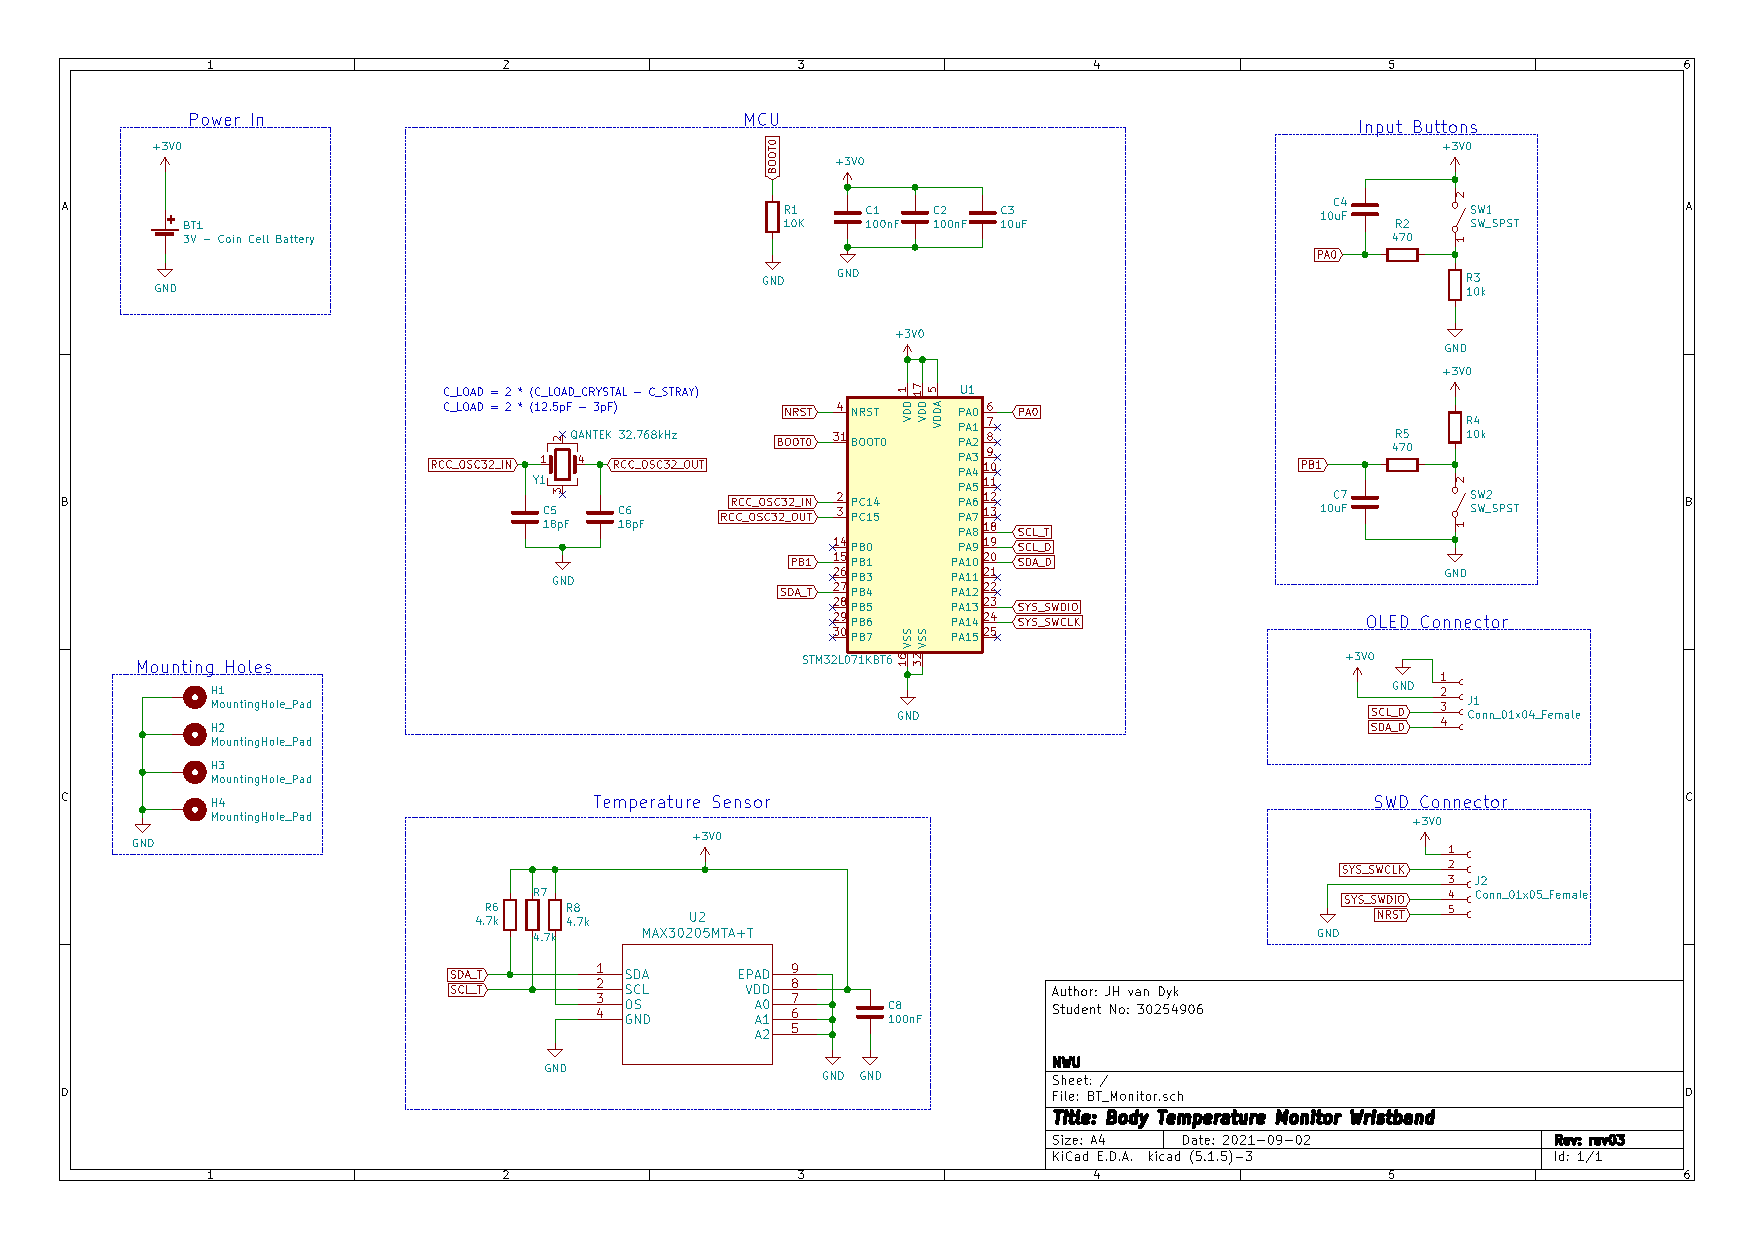
\includegraphics[scale=0.7, angle=90]{img/Schematic}
	\caption{Full schematic of device}
\end{figure}

\chapter{Accuracy Experiment Data}\label{Exp-Data}
\section{Skin Temperature}
\begin{figure}[H]
	\centering
	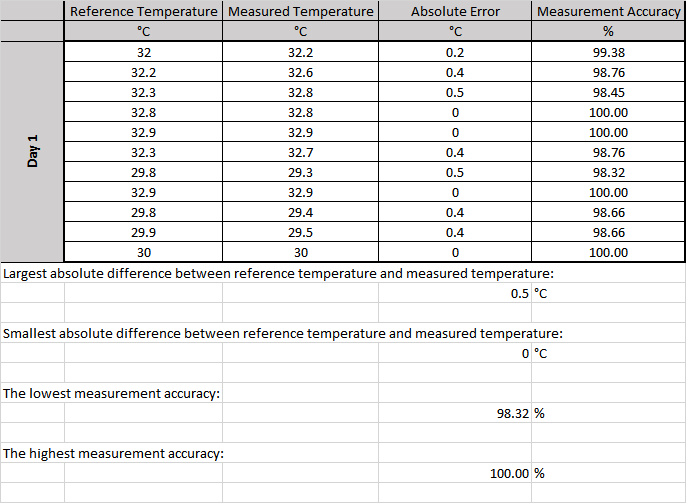
\includegraphics[scale=0.7]{img/Skin-Temp-Data.png}
	\caption{Accuracy of Skin Temperature Measurement Data}
\end{figure}

\section{Body Temperature}
\begin{figure}[H]
	\centering
	\includegraphics[scale=0.7]{img/Body-Temp-Data.png}
	\caption{Accuracy of Body Temperature Measurement Data}
\end{figure}
\end{document}